\documentclass[11pt,a4paper,draft]{report}

% =========================================================
% PACKAGES
% =========================================================

\usepackage{times}
\usepackage{graphicx}

\tolerance=1
\emergencystretch=\maxdimen
\hyphenpenalty=10000
\hbadness=10000

\usepackage{amsmath}
\usepackage{longtable}
\usepackage{acro}
\usepackage[utf8]{inputenc}

%\usepackage[acronym]{glossaries}
%\usepackage[toc]{glossaries}
%\usepackage[refpage]{nomencl}

\usepackage{color}
\usepackage{amssymb}
\usepackage{caption}
\usepackage{subcaption}
\usepackage{txfonts}
\usepackage{mathdots}
\usepackage{rotating}
\usepackage{array}
\usepackage[classicReIm]{kpfonts}

%\usepackage[dvips]{graphicx}

\DeclareGraphicsExtensions{.pdf,.jpeg,.png,.PNG}

% =========================================================
% HYPERREF
% =========================================================

\PassOptionsToPackage{hyphens}{url}

\usepackage{hyperref}

\hypersetup{
    colorlinks=true,
    linkcolor=blue,
    filecolor=magenta,
    urlcolor=cyan,
    citecolor={red}
}

\urlstyle{same}

% =========================================================
% MATHEMATICS / REFERENCES
% =========================================================

\usepackage{mathtools}
\usepackage[superscript]{cite}

% =========================================================
% PAGE FORMAT
% =========================================================

\usepackage[
    top=2cm,
    bottom=2cm,
    left=2.5cm,
    right=2cm
]{geometry}

\usepackage[compact]{titlesec}

\usepackage{fancyhdr}
\usepackage{setspace}
\usepackage{fontenc}
\usepackage{microtype}

% =========================================================
% TABLES
% =========================================================

\usepackage{booktabs}
\usepackage{multirow}
\usepackage[table,xcdraw]{xcolor}

\setlength{\arrayrulewidth}{0.4mm}
\setlength{\tabcolsep}{18pt}
\renewcommand{\arraystretch}{1.5}

% =========================================================
% WATERMARK
% =========================================================

% Temporarily disabled because it was causing
% graphicx package option clash.
%
% \usepackage[printwatermark]{xwatermark}
% \usepackage{transparent}

% =========================================================
% ALGORITHMS
% =========================================================

\usepackage{algorithm2e}
\usepackage{algorithm}
\usepackage[noend]{algpseudocode}

% =========================================================
% PDF / SYMBOLS
% =========================================================

\usepackage[final]{pdfpages}

% Temporarily disabled to avoid possible font conflicts.
% Uncomment later if your document specifically needs them.
%
% \usepackage{MnSymbol,wasysym}

% =========================================================
% TIKZ
% =========================================================

\usepackage{tikz}
\usetikzlibrary{positioning,calc}

% =========================================================
% HEADER / FOOTER
% =========================================================

\pagestyle{fancy}

\fancyhf{}

\fancyhead[R]{\itshape\leftmark}

\fancyfoot[C]{\thepage}

\renewcommand{\headrulewidth}{0pt}

% =========================================================
% FONT / LINE SPACING
% =========================================================

\usepackage{mathptmx}

\linespread{1.5}

% =========================================================
% DOCUMENT
% =========================================================

\begin{document}

% ---------------------------------------------------------
% FRONT MATTER
% ---------------------------------------------------------

\renewcommand{\thepage}{\roman{page}}

% TITLE PAGE
\thispagestyle{empty}
%\addcontentsline{toc}{chapter}{Cover Page}\index{Cover Page}
\begin{center}
\setstretch{2}
\textcolor{purple}{{\huge \textsc{AI - driven Women’s reproductive Health & Risk Awareness
} }}\\
A Project Report \\
\vspace{0.3cm}
Submitted By\\
\vspace{0.1cm}
\textcolor{olive}{{\Large \bf Dhvani Milin Chokshi - 2303031050127}\\
{\Large \bf }}\\
\vspace{0.1cm}
\textcolor{olive}{{\Large \bf Siddhi Chiragbhai Upadhyay - 2303031050657}\\
{\Large \bf }}\\
\vspace{0.1cm}
\textcolor{olive}{{\Large \bf Kashish Mayur Shah - 2303031050547}\\
{\Large \bf }}\\
\vspace{0.1cm}
\textcolor{olive}{{\Large \bf Krusha Maheshbhai Paghadal - 2303031050320}\\
{\Large \bf }}\\
\vspace{0.1cm}
in Partial Fulfilment For the Award of\\
the Degree of\\
BACHELOR OF TECHNOLOGY\\
COMPUTER SCIENCE AND ENGINEERING\\
Under the Guidance of\\
\large{\textbf{Prof. Nidhi Mam}}\\
Your Guide Designation\\

\vspace{0.3cm}
\begin{figure}[h]
\begin{center}
     
\includegraphics[scale=0.18]{parullogo.png} \\
     \vspace{0.7cm}
     \includegraphics[scale=0.02]{Digital Use - PU NAAC Logo.jpg}
\end{center}
\end{figure}
%\textcolor{teal}{\textbf{\Huge{PARUL UNIVERSITY \\ %\textbf{NAAC A++}}}}\\
VADODARA\\
November - 2026
\end{center}


%\include{Chap-3}

\thispagestyle{plain}
\setstretch{1.5}
%\fontfamily{qag}\selectfont
\begin{figure}
    \centering
    
\includegraphics[scale=0.15]{parullogo.png}
    \end{figure}
\vspace{1.5cm}
\begin{center}
    {\Huge \textsc{\color{violet}PARUL UNIVERSITY}}\\
   
    \vspace{1cm}
     {\Huge \bf \textsc{\color{teal}Certificate}}\\
     \vspace{0.5cm}
     \end{center}
     \large{This is to Certify that Project - II (303105423) of $7^{th}$ Semester entitled  " FemCare : AI - driven Women’s reproductive Health \& Risk Awareness ” of Group No. CSE\_35 has been successfully completed by}
     \begin{center}
\large
\begin{tabular}{l@{\hspace{6cm}}r}
Dhvani Milin Chokshi & 2303031050127\\[0.05cm]
Siddhi Chiragbhai Upadhyay & 2303031050657\\[0.05cm]
Kashish Mayur Shah & 2303031050547\\[0.05cm]
Krusha Maheshbhai Paghadal & 2303031050320
\end{tabular}
\end{center}
     \noindent
    \large {under my guidance in partial fulfillment of the Bachelor of Technology (B.Tech) in Computer Science and Engineering of Parul University in Academic Year 2026- 2027.}\\ \par
   \vspace{0.5cm}
    Date of Submission :\_\_\_\_\_\_\_\_\_\_\_\_\_\_\_\_\_\_
   
 \vspace{1.0cm}

\begin{center}
\begin{tabular*}{\textwidth}{@{\extracolsep{\fill}} c c c @{}}

\color{brown}\textbf{Prof. Nidhi Patel } &
\color{brown}\textbf{Prof. Namrata Patel} &
\color{brown}\textbf{Dr. Shailendra K Mishra} \\[0.3cm]

\textbf{Project Guide} &
\textbf{Project Coordinator} &
\textbf{Head of Department} \\[0.3cm]

\textbf{CSE, PIET} &
\textbf{CSE, PIET} &
\textbf{CSE, PIET} \\

\textbf{Parul University} &
\textbf{Parul University} &
\textbf{Parul University}

\end{tabular*}
\end{center}
   
   

%ACKNOLEDGEMENT PAGE
\thispagestyle{empty}
\newpage
\cleardoublepage\phantomsection
\addcontentsline{toc}{chapter}{Acknowledgements}\index{Acknowledgements}
\begin{center}
{\Large \bf Acknowledgements}\\
\end{center}
\vspace{10pt}
\begin{flushright}
\textit{“The single greatest cause of happiness is gratitude.” }\\
\vspace{5mm}
-Auliq-Ice
\end{flushright}
\hspace{10mm}Acknowledgements
We express our sincere gratitude to all those who supported and guided us throughout the
successful completion of this project. First and foremost, we are grateful to the Almighty for granting us the strength, wisdom, and determination to carry out this work.
We extend our heartfelt thanks to our project guide, Prof. or Dr. Your Guide Name, for his/her invaluable guidance, continuous encouragement, and constructive feedback at every stage of this project. His/Her expertise and dedication have been a constant source of inspiration.
We are also thankful to the faculty members and staff of the Department of Computer
Science and Engineering, Parul Institute of Engineering and Technology, Parul University, for
providing us with the necessary resources, infrastructure, and academic support.
We sincerely thank Dr. Shailendra K Mishra, Head of Department, CSE, PIET, Parul
University, for his support and leadership. 
Finally, we are deeply grateful to our parents, family members, and well-wishers for their
constant moral support and motivation throughout this journey.

\vspace{1.5cm}
\begin{flushright}
\textbf{Dhvani milin Chokshi \\ CSE, PIET\\ Parul University, \\Vadodara}\\ 
\end{flushright}

\thispagestyle{empty}
\newpage
\cleardoublepage\phantomsection
\addcontentsline{toc}{chapter}{Abstract}\index{Abstract}
\begin{center}
{\Large \bf Abstract}\\
\end{center}
\vspace{10pt}

Women's reproductive health conditions, including Polycystic Ovary Syndrome (PCOS), irregular menstrual cycles, and related hormonal disorders, are prevalent yet frequently identified late due to limited health awareness and fragmented access to specialised care. Existing digital cycle-tracking tools enable basic period logging but do not offer structured risk screening, intelligent health guidance, or integration with local healthcare providers. This project presents FEMCARE, a full-stack web application that provides women with an integrated platform for reproductive health monitoring, PCOS risk assessment, AI-assisted health information, and healthcare appointment management.

FEMCARE is built on a React and Vite frontend, a Python FastAPI backend, and a Supabase-managed PostgreSQL cloud database. The system implements an 18-feature PCOS risk screening module using a pre-trained XGBoost machine learning classifier that processes user-reported clinical indicators -- covering cycle regularity, physical symptoms, lifestyle factors, and optional hormonal values -- and returns a risk classification of Low, Moderate, or High Risk with a confidence percentage. A heuristic fallback ensures continued functionality when the model is unavailable. An AI health assistant, powered by the Groq large language model API, is constrained to women's reproductive health topics through a two-layer mechanism combining a Python keyword filter and an LLM system prompt, with responses enriched by the authenticated user's real cycle and symptom data. An appointment booking module displays ten women's healthcare providers in Vadodara on an interactive map, manages sixteen daily time slots per provider, and enforces double-booking prevention through a PostgreSQL partial unique index. Appointment confirmation and cancellation emails are delivered via the Resend API, and all user health data is protected by Row Level Security policies at the database level.

FEMCARE demonstrates the practical integration of machine learning, large language model assistance, cloud database management, and modern web technologies within a secure, clinically responsible women's health platform. The system is intended as a screening and awareness tool and does not replace professional medical diagnosis.

\vspace{10pt}
\noindent\textbf{Keywords:} Women's Health, PCOS Detection, Menstrual Cycle Tracking, XGBoost, Large Language Model, FastAPI, Supabase, React, Appointment Booking, Row Level Security


\begin{spacing}{2}
\newpage
\cleardoublepage\phantomsection
%\addcontentsline{toc}{chapter}{Table of Contents}%\index{Contents}
\renewcommand*\contentsname{Table of Contents}
\tableofcontents
\end{spacing}

\begin{doublespace}
\newpage
\pagestyle{empty}
\cleardoublepage\phantomsection
\addcontentsline{toc}{chapter}{List of Tables} 

\listoftables

\cleardoublepage\phantomsection
\addcontentsline{toc}{chapter}{List of Figures}

\listoffigures 
\end{doublespace}
\clearpage\phantomsection
%\addcontentsline{toc}{chapter}{List of Abbreviations}
%\includepdf[pages=-]{ListofAbbreviations.pdf}




% ---------------------------------------------------------
% MAIN MATTER
% ---------------------------------------------------------

\pagenumbering{arabic}

% Chapter header
\renewcommand{\chaptermark}[1]{%
    \markboth{\chaptername\ \thechapter\ -\ #1}{}%
}

\pagestyle{fancy}

\renewcommand{\headrulewidth}{2pt}

\renewcommand{\footrulewidth}{1pt}

% ---------------------------------------------------------
% CHAPTERS
% ---------------------------------------------------------

% ============================================================
% CHAPTER 1 -- INTRODUCTION
% FEMCARE: An AI-Powered Women's Reproductive Health Platform
% ============================================================

\chapter{Introduction}\doublespacing
\label{chap:introduction}

\section{Background}
\label{sec:background}

Women's reproductive health conditions -- including Polycystic Ovary Syndrome (PCOS), irregular menstrual cycles, and related hormonal disorders -- are prevalent yet frequently identified late due to limited health awareness and fragmented access to specialist care. Existing digital tools allow basic period logging but provide no structured risk screening, no domain-specific health guidance, and no integration with local healthcare providers. \cite{epstein2017}\cite{ahmed2023}

Advances in machine learning and large language models (LLMs) have made it practical to build web-based platforms that offer clinical risk screening from user-reported data and intelligent, scoped health assistance. \cite{zad2024}\cite{maity2025} Deploying such a platform as a web application makes it accessible without installation, which is particularly relevant for users in semi-urban regions such as Vadodara, Gujarat, where specialist gynaecological services may not be immediately accessible.

% ------------------------------------------------------------
\section{Problem Statement}
\label{sec:problem}

No unified digital platform currently provides women with cycle tracking, structured PCOS risk assessment, topic-restricted AI health guidance, and local provider booking in a single authenticated application. \cite{epstein2017}\cite{kim2024} Users must rely on multiple disconnected tools, receive no risk indication from their logged data, and have no digital means to locate or book local women's health consultations. Personal health data stored by lightweight apps often lacks database-level per-user isolation. \cite{kotz2016} FEMCARE is proposed to address these gaps.

% ------------------------------------------------------------
\section{Proposed Solution}
\label{sec:solution}

FEMCARE is a full-stack web application providing an integrated platform for women's reproductive health monitoring, PCOS risk assessment, AI-assisted health guidance, and healthcare provider booking. The major implemented components are:

\begin{itemize}
    \item \textbf{Menstrual Cycle Tracking:} Daily logging of flow, pain level, mood, and symptoms, persisted in a cloud PostgreSQL database.
    \item \textbf{PCOS Risk Assessment:} An 18-feature guided assessment processed by a pre-trained XGBoost classifier, returning a Low, Moderate, or High Risk classification with a confidence percentage.
    \item \textbf{AI Health Assistant:} A Groq LLM-powered chatbot restricted to women's reproductive health topics, enriched with the authenticated user's real health data.
    \item \textbf{Find Care and Booking:} An interactive map of 10 Vadodara providers with 16 daily time slots, database-level double-booking prevention, and email confirmation via the Resend API.
    \item \textbf{Health Awareness:} Educational content for 8 reproductive health conditions with search and category filtering.
    \item \textbf{Dashboard:} Real-time cycle phase display, logged health summary, and compact AI assistant.
    \item \textbf{Security:} Supabase Authentication with JWT tokens; Row Level Security on all user data tables.
\end{itemize}

% ------------------------------------------------------------
\section{Aim and Objectives}
\label{sec:aim}

The aim of this project is to design and implement a secure, AI-powered women's reproductive health web application that integrates cycle tracking, PCOS risk screening, health guidance, provider booking, and educational awareness in a single platform.

The specific objectives are:

\begin{enumerate}
    \item Implement secure user authentication and automatic profile creation via a PostgreSQL trigger.
    \item Develop a daily cycle logging module with cloud persistence and Dashboard synchronisation.
    \item Build an 18-feature PCOS risk screening module using a pre-trained XGBoost classifier with a heuristic fallback.
    \item Implement a topic-restricted AI health assistant using the Groq LLM API with user-context enrichment.
    \item Develop a provider booking module with slot management and database-enforced double-booking prevention.
    \item Send transactional appointment emails via the Resend API.
    \item Create a searchable Women's Health Awareness module covering 8 conditions.
    \item Enforce Row Level Security on all user data tables in Supabase PostgreSQL.
\end{enumerate}

% ------------------------------------------------------------
\section{Scope}
\label{sec:scope}

FEMCARE is implemented as a web application covering cycle tracking, PCOS assessment, AI chat, Find Care and booking, health awareness, period history, and symptom history. The subscription plan page is a UI comparison only -- no payment integration is implemented. Wearable device integration, telemedicine, and a native mobile application are outside the current scope.

% ------------------------------------------------------------
\section{Organisation of the Thesis}
\label{sec:organisation}

\begin{itemize}
    \item \textbf{Chapter 2 -- Literature Survey:} Reviews related work in women's digital health, PCOS detection, and AI health assistants.
    \item \textbf{Chapter 3 -- SRS:} Defines functional and non-functional requirements.
    \item \textbf{Chapter 4 -- System Design:} Covers architecture, database design, and data flows.
    \item \textbf{Chapter 5 -- Methodology:} Describes the implementation of each component.
    \item \textbf{Chapter 6 -- Implementation:} Presents functional test cases and observed results.
    \item \textbf{Chapter 7 -- Conclusion:} Summarises the completed work.
    \item \textbf{Chapter 8 -- Future Scope:} Proposes realistic enhancements.
\end{itemize}


\chapter{Literature Survey}
\doublespacing

\section{Introduction}

The literature survey focuses on recent advancements in AI and machine learning for women's healthcare, including menstrual cycle prediction, PCOS detection, and reproductive health monitoring. Various models such as LSTM, XGBoost, and Random Forest have been widely used for accurate prediction and classification. Some studies also explore AI-based chatbots, IoT systems, and telemedicine platforms to improve accessibility and user engagement. Privacy-preserving approaches like federated learning are introduced to protect sensitive health data. However, many existing systems lack integration, real-time monitoring, and personalization. Additionally, issues like small datasets, limited generalization, and lack of explainability remain. These gaps highlight the need for a secure, scalable, and intelligent healthcare solution.

\section{Critical Evaluation of Research Papers}

This section provides a detailed evaluation of all twenty research papers reviewed, examining their contributions, methodologies, and limitations.

\subsection{Paper 1: A Generative Predictive Model for Menstrual Cycle Lengths (2021)}
In this paper, Kathy Li et al. (2021) introduced a generative predictive model for predicting menstrual cycle lengths based on self-tracked mobile health data. The model includes hierarchical structures to handle missing or inconsistent user information and to separate biological signals from tracking artifacts. The model allows for continuous updating and personalization. The proposed method is more accurate than previous ones for predicting menstrual cycle lengths, but it is based on user information and may therefore be biased. \cite{li2021,urteaga2017,li2020}\cite{urteaga2017}\cite{li2020}

\subsection{Paper 2: AI-Based Menstrual Cycle Tracking and Health Assistant (2025)}
An AI-based system for tracking the menstrual cycle using the LSTM algorithm for prediction and Isolation Forest for anomaly detection has been proposed by Anand Kharode et al. in their paper (2025). A chatbot has also been integrated using NLP, which increases the level of engagement and accuracy of the prediction. The proposed system has been developed using the MERN stack, thus ensuring the scalability of the application. However, the privacy of the data has also raised certain concerns. \cite{soni2025}

\subsection{Paper 3: PCOS Disease Classification Using XGBoost (2025)}
In this paper, Atika et al. proposed a machine learning model based on XGBoost, combined with genetic algorithms and SMOTE for classification. The proposed model improves the precision of the classification results and is capable of handling imbalanced data. However, this model may not perform well in different populations. \cite{ahmed2023}

\subsection{Paper 4: Examining Menstrual Tracking to Inform Design (2017)}
Daniel A. Epstein et al. (2017) conducted a study on menstrual tracking using surveys and user feedback. This study provides information on user behavior, user motivation, and the limitations of existing systems. This study highlights the problem of inaccurate predictions and the need for more inclusive designs. This study provides useful insights for designing better applications. This study does not provide any predictive model. \cite{epstein2017,liu2019}

\subsection{Paper 5: Federated AI Framework for Menstrual Health Prediction (2025)}
M. Rajesh (2025) proposed a federated AI system using contactless biosensing for menstrual prediction. This system provides better privacy and personalization using local data processing. This system provides better accuracy and security for real-time predictions. This system uses multimodal data for better performance. This system requires complex infrastructure and hardware. \cite{rajesh2025}

\subsection{Paper 6: ML Methods for Predicting Depression in Menopausal Women (2023)}
Md. Mamun Ali et al. (2023) proposed ML models like Random Forest and XGBoost for depression prediction. This system provides better evaluation of performance metrics and high accuracy. This system helps in the early detection of depression. This study compares different models effectively. This study deals with menopausal women only. \cite{ali2023,isayev2023}

\subsection{Paper 7: Prediction of Fertile Window Using ML (2022)}
In the paper by Jia-Le Yu et al. (2022), the authors used physiological data for prediction. The model has good performance for predicting the fertile window and the menstrual cycles. The model has good performance for individuals with regular cycles. Clinical validation also improves the reliability of the model. However, the performance of the model is not good for individuals with irregular cycles. \cite{yu2022,goodale2019}

\subsection{Paper 8: AI-Based Thermographic Monitoring (2025)}
In the paper by Lucas M. Iturriago-Salas et al. (2025), the authors proposed an AI-driven mobile platform for thermographic maternal health monitoring. The proposed system uses deep learning algorithms on mobile devices such as smartphones. The proposed system has good performance for improving the usability of the system in the healthcare sector. However, the performance of the proposed system is limited by the quality of the image. \cite{iturriago2025}

\subsection{Paper 9: IoT-Based Mobile Health Architecture (2024)}
Ana Gonz\'{a}lez Berm\'{u}dez et al. proposed a scalable mHealth architecture through data fusion and IoT in 2024. The system is useful for developing modular and reusable applications in healthcare. The system is effective for improving interoperability and efficiency. The proposed architecture is applicable to different use cases. However, there is no specific example of implementation. \cite{kilungeja2025}

\subsection{Paper 10: AI Chatbots in Women's Health (2024)}
Hyun-Kyoung Kim presented research on the effects of AI chatbots on women's health in 2024. The study demonstrates positive effects on mental health and users' engagement. Chatbots offer interactive and scalable solutions for users. Chatbots improve the accessibility of healthcare services. However, reliability and accuracy are major concerns. \cite{kim2024}

\subsection{Paper 11: Privacy and Security in Mobile Health Systems (2016)}
David Kotz et al. (2016) studied the security challenges faced by the mobile health system. The paper discusses the risks faced by the system, including data breaches and vulnerabilities. It also emphasizes the significance of protecting the privacy of the users. The handling of the data by the system is of utmost importance, as it can create a sense of trust among the users. However, the paper fails to provide solutions to the problem. \cite{kotz2016}

\subsection{Paper 12: ML Model Comparison for Menstrual Prediction (2025)}
Mutiara Khairunisa et al. (2025) presented a paper that compared the three models, including the LSTM, CNN, and Decision Tree models, for the prediction of the menstrual cycle. The paper shows that the highest accuracy is obtained by the LSTM model, as it can track the patterns of the data. However, the dataset used for the research is small. \cite{khairunisa2025,rego2023}

\subsection{Paper 13: PCOS Prediction Using EHR (2024)}
Zahra Zad et al. (2024) suggested the implementation of machine learning models using EHRs for PCOS prediction. The system uses clinical data such as hormone levels. It provides high prediction accuracy. It can be used for early diagnosis. However, it depends on the availability of EHRs. \cite{zad2024}

\subsection{Paper 14: High-Risk Pregnancy Prediction Using ML (2025)}
Xinyu Pi et al. (2025) implemented machine learning algorithms for predicting high-risk pregnancy. The researchers used multiple classifiers. MLP showed the best results. It provides high accuracy. It can be used for early identification. However, it should be tested using different datasets. \cite{pi2025}

\subsection{Paper 15: Explainable AI in Healthcare (2025)}
Qaiser Abbas et al. (2025) discussed the implementation of explainable AI in clinical decision support systems. It highlights the importance of explainability in AI. It also discusses different techniques used in clinical decision support systems. Explainability helps in making AI more reliable. However, its implementation in real-life scenarios is lacking. \cite{abbas2025}

\subsection{Paper 16: Review of PCOS Detection Techniques (2023)}
The paper presented by Samia Ahmed et al. (2023) is a review-based paper on the detection of PCOS using machine learning algorithms. The paper discusses the performance of algorithms like CNN, SVM, Random Forest, and LR on different datasets. The paper also discusses the limitations of the algorithms, like class imbalance and the unavailability of a standard dataset for PCOS detection. However, the paper does not propose a new model for the detection of PCOS. \cite{ahmed2023}

\subsection{Paper 17: Web-Based ML for PCOS Prediction (2024)}
In the paper titled ``Empowering Early Detection: Web-Based ML Approach for PCOS Prediction'' by Md. Mahbubur Rahman et al. (2024), the author has proposed a web-based approach for the early detection of PCOS using machine learning approaches. The proposed approach has utilized feature selection techniques such as ``Mutual Information'' for better prediction accuracy. The proposed approach has also utilized multiple classifiers such as Random Forest, AdaBoost, and SVM. The proposed approach has also demonstrated high accuracy for the prediction of PCOS. \cite{rahman2024}

\subsection{Paper 18: AI-Based Women's Health Monitoring (2025)}
This paper proposes an AI-driven system for monitoring women's reproductive health and predicting potential disorders using machine learning techniques. The system integrates health parameters such as menstrual patterns, symptoms, and physiological data to provide early risk prediction. It uses supervised learning models to improve prediction accuracy and support decision-making. A key strength is its focus on personalized healthcare and real-time monitoring. However, the system depends on data quality and user input reliability. Overall, it is relevant for developing intelligent healthcare platforms for women's health. \cite{maity2025}

\subsection{Paper 19: AI in Telemedicine (2025)}
Martina Rossi et al. (2025) have presented a systematic review of AI in telemedicine across various domains of healthcare. The paper has mentioned the usage of AI in diagnostics, patient monitoring using wearables, and chatbots in delivering healthcare services. It has also been mentioned that AI can be used to increase the accuracy of diagnostics and to deliver real-time healthcare services. However, there are also challenges that need to be overcome in using AI in telemedicine. The paper has emphasized the importance of AI in delivering telemedicine services. \cite{rossi2025}

\subsection{Paper 20: LLMs in Healthcare (2025)}
Subhankar Maity et al. (2025) have presented a comprehensive review of LLMs in delivering healthcare services. The paper has mentioned the usage of LLMs in delivering clinical decisions, diagnostics, medical education, and patient communication. It has also been mentioned that LLMs can be used to increase the efficiency and knowledge of patients. However, there are also challenges that need to be overcome in using LLMs. The paper has emphasized the importance of LLMs in delivering future AI-driven intelligent healthcare services. \cite{maity2025,wang2024}


\section{Existing Research Paper on Learning}

A significant amount of research has been conducted to enhance privacy and security in federated learning systems. Various techniques such as differential privacy, secure aggregation, and encryption are widely explored to protect sensitive data. Researchers have also analyzed vulnerabilities like data poisoning and inference attacks. These studies aim to improve the reliability and robustness of distributed learning models. The following table summarizes key contributions in this domain.

\begin{center}
\small
\setlength{\tabcolsep}{6pt}
\renewcommand{\arraystretch}{1.2}

\begin{longtable}{|c|p{3cm}|c|p{3.5cm}|p{3cm}|p{3cm}|}
\hline
Sr. & Author & Year & Summary & Advantages & Disadvantages \\
\hline
\endfirsthead

\hline
Sr. & Author & Year & Summary & Advantages & Disadvantages \\
\hline
\endhead

1 & Kathy Li et al. \cite{li2021} & 2021 & Predictive menstrual cycle model & Personalized predictions & Biased data \\
2 & Anand Kharode et al. \cite{soni2025} & 2025 & AI menstrual tracking (LSTM) & Scalable system & Privacy issues \\
3 & Atika et al. \cite{ahmed2023} & 2025 & PCOS classification (XGBoost) & Handles imbalance & Limited generalization \\
4 & Daniel Epstein et al. \cite{epstein2017} & 2017 & Menstrual tracking study & Design insights & No prediction \\
5 & M. Rajesh \cite{rajesh2025} & 2025 & Federated AI health system & High privacy & Complex system \\
6 & Md. Mamun Ali et al. \cite{ali2023} & 2023 & Depression prediction ML & High accuracy & Limited group \\
7 & Jia-Le Yu et al. \cite{yu2022} & 2022 & Fertile window prediction & Good for regular cycles & Poor irregular cycles \\
8 & Lucas Iturriago et al. \cite{iturriago2025} & 2025 & AI thermographic monitoring & Mobile-friendly & Image quality issues \\
9 & Ana Berm\'{u}dez et al. \cite{kilungeja2025} & 2024 & IoT health architecture & Scalable & No implementation \\
10 & Hyun-Kyoung Kim \cite{kim2024} & 2024 & AI chatbots study & Better engagement & Accuracy issues \\
11 & David Kotz et al. \cite{kotz2016} & 2016 & Security in mobile health & Highlights risks & No solutions \\
12 & Mutiara Khairunisa \cite{khairunisa2025} & 2025 & ML comparison (LSTM best) & High accuracy & Small dataset \\
13 & Zahra Zad et al. \cite{zad2024} & 2024 & PCOS using EHR & Early diagnosis & Depends on EHR \\
14 & Xinyu Pi et al. \cite{pi2025} & 2025 & High-risk pregnancy ML & Early detection & Needs validation \\
15 & Qaiser Abbas et al. \cite{abbas2025} & 2025 & Explainable AI & Trust improvement & Limited use \\
16 & Samia Ahmed et al. \cite{ahmed2023} & 2023 & PCOS ML review & Comprehensive & No new model \\
17 & Md. Rahman et al. \cite{rahman2024} & 2024 & Web ML PCOS system & Accurate & Needs testing \\
18 & Sarvesh Gupta et al. \cite{maity2025} & 2025 & AI health monitoring & Personalized & Data dependency \\
19 & Martina Rossi et al. \cite{rossi2025} & 2025 & AI in telemedicine & Better diagnosis & Challenges exist \\
20 & Subhankar Maity et al. \cite{maity2025} & 2025 & LLM healthcare review & Efficient & Ethical issues \\
\hline
\caption{Summary of Existing Research on Learning with Privacy (Papers 1--20)}
\end{longtable}
\end{center}

\section{Critical Evaluation of Existing Research}
\label{sec:critical-eval}

The reviewed literature demonstrates meaningful progress in applying machine learning and AI to women's reproductive health, yet several recurring limitations motivate the development of an integrated platform such as FemCare.

\textbf{Strengths of Existing Approaches.}
Multiple studies confirm that machine learning models are effective for menstrual cycle prediction and PCOS detection. Generative and hierarchical models applied to self-tracked mHealth data have shown state-of-the-art performance for personalised cycle-length prediction \cite{li2021,urteaga2017,li2020}. Physiological and wearable-sensor data have been used to predict fertile windows and detect menstrual phase transitions \cite{yu2022,goodale2019,kilungeja2025}. Gradient-boosted models, including XGBoost, have demonstrated high classification accuracy for PCOS when trained on clinical or EHR datasets \cite{ahmed2023,zad2024,rahman2024}. LLMs and AI chatbots have been shown to produce positive health outcomes in women's health contexts \cite{maity2025,wang2024,kim2024}, while systematic reviews of AI in telemedicine and clinical decision support confirm the broader applicability of these technologies \cite{rossi2025,abbas2025}.

\textbf{Dataset and Population Limitations.}
A consistent limitation across the reviewed studies is the use of small or homogeneous datasets. Several menstrual prediction models were evaluated on datasets that are too limited to generalise across populations with irregular cycles \cite{khairunisa2025,rego2023,li2021}. PCOS prediction models relying on EHR data are restricted to populations that interact with the healthcare system and cannot be applied to community-based screening \cite{zad2024}. High-risk pregnancy prediction models similarly require validation on independent and diverse datasets before clinical application \cite{pi2025}. Studies focused on menopausal or postmenopausal populations \cite{ali2023,isayev2023} further illustrate that findings from one reproductive-age group do not automatically generalise to others.

\textbf{Personalization and Longitudinal Tracking.}
Existing tracking applications demonstrate the importance of self-tracked data for personalised predictions \cite{epstein2017,liu2019}, yet most lack adaptive models that update continuously as new data is recorded. Personalised hormonal-cycle models that separate biological signals from tracking artefacts \cite{li2021,urteaga2017} and approaches that characterise individual physiological variation \cite{li2020,goodale2019} remain largely research prototypes without direct clinical integration.

\textbf{Privacy and Security Gaps.}
Privacy-preserving and federated approaches have been proposed to protect sensitive reproductive health data \cite{rajesh2025,kotz2016}. However, as noted by Kotz et al. \cite{kotz2016}, most mHealth systems still lack robust access control and data isolation mechanisms. Lightweight applications commonly store data locally without database-level per-user isolation, creating vulnerabilities that an integrated cloud-backed system with Row Level Security can address.

\textbf{Explainability Limitations.}
Several studies acknowledge that non-linear ensemble models such as XGBoost and neural networks provide limited interpretability \cite{ahmed2023,zad2024}. Abbas et al. \cite{abbas2025} specifically highlight that explainable AI in clinical settings improves trust but remains difficult to deploy in real-world scenarios. Addressing this gap through feature-importance analysis and SHAP-based explanations is identified as future work for FemCare \cite{lundberg2017}.

\textbf{Integration Gaps.}
Despite strong individual results in cycle prediction \cite{li2021,rego2023,khairunisa2025}, PCOS detection \cite{ahmed2023,zad2024,rahman2024}, chatbot health support \cite{kim2024,maity2025}, and AI-assisted monitoring \cite{iturriago2025,soni2025}, no existing system integrates all of these capabilities alongside healthcare-provider discovery and appointment booking within a single authenticated platform. The FemCare dataset \cite{dataset} was developed specifically to support an integrated prediction and awareness system targeting this gap in women's health technology.

\section{Research Gap}

The available research on women's healthcare is primarily focused on solving individual problems, such as predicting periods or detecting PCOS. \cite{dataset} However, no comprehensive framework is available. Some methods rely on limited data, causing them to be less accurate. Real-time monitoring and personalization for irregular cycles are not yet available. Although methods for ensuring user privacy are available, they have not been effectively implemented. Also, no methods for increasing user trust in AI systems have been proposed yet. Integration of state-of-the-art technologies such as LLMs and telemedicine is yet to be effectively implemented.

% ============================================================
% CHAPTER 3 -- ANALYSIS / SOFTWARE REQUIREMENTS SPECIFICATION
% FEMCARE: An AI-Powered Women's Reproductive Health Platform
% ============================================================

\chapter{Analysis / Software Requirements Specification (SRS)}\doublespacing
\label{chap:srs}

% ------------------------------------------------------------
\section{Introduction}
\label{sec:srs-intro}

This chapter documents the system analysis and software requirements for FEMCARE. It identifies the limitations of existing systems that FEMCARE is designed to address, establishes the user requirements derived from the intended application, and specifies the functional and non-functional requirements that governed the system's development. The feasibility and constraints of the project are also considered. Architectural design, implementation details, and testing procedures are covered in subsequent chapters.

% ------------------------------------------------------------
\section{Existing System and its Limitations}
\label{sec:existing}

Current digital tools for women's reproductive health fall broadly into two categories: cycle-tracking applications and general-purpose health information services. While cycle-tracking applications allow users to record period dates and flow intensity, they provide no structured clinical risk screening, and their outputs are limited to predicted period dates and general cycle statistics. \cite{epstein2017}\cite{li2021} A user whose logs indicate patterns associated with PCOS -- such as irregular cycles, excess facial hair, or skipped periods -- receives no risk indication from such tools. \cite{zad2024}\cite{ahmed2023}

General-purpose AI assistants are not restricted to women's health and cannot tailor responses to a user's personal health history. \cite{kim2024} Appointment booking for women's health consultations in cities such as Vadodara typically requires telephone contact or direct walk-in visits. No unified digital platform currently provides cycle tracking, structured PCOS risk screening, scoped health guidance, and local provider booking in a single authenticated application. The key limitations motivating FEMCARE are summarised in Table~\ref{tab:existing-limitations}.

\begin{table}[h!]
\centering
\caption{Limitations of Existing Systems and How FEMCARE Addresses Them}
\label{tab:existing-limitations}
\renewcommand{\arraystretch}{1.4}
\begin{tabular}{|p{4.2cm}|p{8.1cm}|}
\hline
\rowcolor[HTML]{D9D9D9}
\textbf{Limitation of Existing Systems} & \textbf{Description} \\
\hline
No integrated PCOS assessment &
Existing cycle-tracking applications primarily record menstrual data but do not provide a structured assessment based on relevant health and clinical inputs. FEMCARE provides an 18-feature assessment that evaluates the entered parameters and returns a PCOS risk result with a confidence measure. \\
\hline
No domain-restricted AI health assistance &
General-purpose AI assistants are not constrained to women's reproductive health and cannot personalise responses using the user's own health data. FEMCARE provides an AI assistant restricted to this domain, enriched with the authenticated user's real cycle and symptom information. \\
\hline
No digital appointment booking for local providers &
Booking a women's health consultation in cities such as Vadodara typically requires telephone contact or walk-in visits. FEMCARE provides online slot booking for ten local providers with automated confirmation and cancellation emails. \\
\hline
No integrated reproductive health awareness &
Health information on conditions such as endometriosis, fibroids, and cervical health is not integrated within existing tracking tools. FEMCARE includes a searchable awareness module covering eight reproductive health conditions, warning signs, and prevention guidance. \\
\hline
Absence of database-level user data isolation &
Lightweight tracking applications often store data locally or rely on application-layer filtering without enforcing per-user access controls at the database level. FEMCARE applies Row Level Security policies in PostgreSQL, ensuring that each user can access only their own data. \\
\hline
\end{tabular}
\end{table}

% ------------------------------------------------------------
\section{Proposed System Overview}
\label{sec:proposed}

FEMCARE is proposed as an authenticated, cloud-backed web application that integrates menstrual cycle tracking, an 18-feature PCOS risk assessment module, a topic-restricted AI health assistant, healthcare provider discovery and booking, and educational health awareness content. All user data is stored in a Supabase-managed PostgreSQL database with Row Level Security policies enforced at the database level. The system is designed as a screening and awareness platform and explicitly does not replace professional medical diagnosis or consultation.

% ------------------------------------------------------------
\section{User Requirements}
\label{sec:user-req}

Based on the intended user group and the implemented application, the following user requirements were identified:

\begin{enumerate}
    \item \textbf{Authentication:} Users must be able to register with a name, email address, password, age, average cycle length, and last period date, and subsequently log in and out securely.

    \item \textbf{Cycle and Symptom Logging:} Users must be able to record daily menstrual data including flow type, pain level, mood, and symptoms for any selected date.

    \item \textbf{Dashboard Overview:} Users must be able to view their current cycle day, phase, recent logged health data, and a navigable monthly calendar from a single screen.

    \item \textbf{PCOS Risk Assessment:} Users must be able to complete a guided health assessment that collects clinical indicators and returns a risk classification with a confidence measure.

    \item \textbf{AI Health Guidance:} Users must be able to ask health questions and receive educational responses within the domain of women's reproductive health.

    \item \textbf{Provider Discovery and Booking:} Users must be able to view local healthcare providers on a map, check slot availability, book an appointment, and cancel a booking.

    \item \textbf{Health Awareness:} Users must be able to browse, search, and filter educational content on reproductive health conditions and warning signs.

    \item \textbf{Profile Management:} Users must be able to view and update their profile information including name, email, cycle length, and last period date.

    \item \textbf{Email Notifications:} Users should receive an email confirmation upon booking or cancelling an appointment.
\end{enumerate}

% ------------------------------------------------------------
\section{Functional Requirements}
\label{sec:functional}

The functional requirements of FEMCARE, derived from the implemented application, are specified in Table~\ref{tab:fr}.

\begin{table}[h!]
\centering
\caption{Functional Requirements}
\label{tab:fr}
\renewcommand{\arraystretch}{1.4}
\begin{tabular}{|p{1.2cm}|p{3.5cm}|p{8cm}|}
\hline
\rowcolor[HTML]{D9D9D9}
\textbf{ID} & \textbf{Requirement} & \textbf{Description} \\
\hline
FR-01 & User Registration & The system shall allow new users to register with name, email, password, age, cycle length, and last period date. \\
\hline
FR-02 & User Authentication & The system shall authenticate users via email and password, establish a persistent session, and redirect unauthenticated requests to the login screen. \\
\hline
FR-03 & Profile Management & Authenticated users shall be able to view and update their profile data stored in the database. \\
\hline
FR-04 & Daily Cycle Logging & Users shall be able to log flow, pain level, mood, and symptoms for any selected date. A unique constraint shall prevent duplicate entries per user per date. \\
\hline
FR-05 & Dashboard Display & The dashboard shall display the current cycle day, phase, a monthly calendar with period and fertility highlights, and the most recently logged health data. \\
\hline
FR-06 & PCOS Assessment & The system shall present an 18-question assessment, automatically calculate the LH/FSH ratio from user-entered values, submit data to the backend, and display the returned risk classification and confidence percentage. \\
\hline
FR-07 & ML-Based Prediction & The backend shall process assessment inputs using a pre-trained XGBoost classifier and return a risk level (Low, Moderate, or High Risk). A heuristic fallback shall be used when the model is unavailable. \\
\hline
FR-08 & AI Health Assistant & The system shall provide a chatbot constrained to women's reproductive health topics. Responses shall be rejected for out-of-scope queries and enriched with the user's real health data when authenticated. \\
\hline
FR-09 & Provider Discovery & The system shall display healthcare providers on an interactive map and as a list, showing name, specialty, address, and contact information. \\
\hline
FR-10 & Appointment Booking & Authenticated users shall be able to book from sixteen daily time slots per provider. The system shall prevent confirmed double-bookings for the same provider, date, and slot. \\
\hline
FR-11 & Booking Management & Users shall be able to view their booking history and cancel a confirmed booking. Cancelled slots shall become available for re-booking. \\
\hline
FR-12 & Email Notifications & The system shall send a confirmation email upon successful booking and a cancellation email upon successful cancellation, including booking details and a booking reference. \\
\hline
FR-13 & Health Awareness & The system shall display educational content on eight reproductive health conditions with search and category filter functionality, and a detail view for each condition. \\
\hline
FR-14 & Period and Symptom History & Users shall be able to view historical period records and symptom log entries. \\
\hline
\end{tabular}
\end{table}

% ------------------------------------------------------------
\section{Non-Functional Requirements}
\label{sec:nonfunctional}

The non-functional requirements governing FEMCARE are specified in Table~\ref{tab:nfr}. The security requirements NFR-01 and NFR-02 reflect established best practices for privacy and data protection in mobile health systems. \cite{kotz2016}

\begin{table}[h!]
\centering
\caption{Non-Functional Requirements}
\label{tab:nfr}
\renewcommand{\arraystretch}{1.4}
\begin{tabular}{|p{1.2cm}|p{3cm}|p{8.5cm}|}
\hline
\rowcolor[HTML]{D9D9D9}
\textbf{ID} & \textbf{Category} & \textbf{Requirement} \\
\hline
NFR-01 & Security & All user health data shall be isolated at the database level using Row Level Security policies, ensuring that no user can access another user's records. \\
\hline
NFR-02 & Security & Passwords shall be managed exclusively by Supabase Authentication. No application table shall store plaintext or hashed passwords. API keys and service credentials shall be stored server-side in environment variables only. \\
\hline
NFR-03 & Reliability & Booking creation shall succeed independently of email delivery. If the email notification service is unavailable, the booking shall remain confirmed and the user shall be informed. \\
\hline
NFR-04 & Reliability & The PCOS assessment shall remain operational through a heuristic fallback when the XGBoost model cannot be loaded. \\
\hline
NFR-05 & Reliability & Frontend API calls shall safely handle non-JSON server responses without application crashes. \\
\hline
NFR-06 & Usability & The application shall be responsive and usable on standard desktop and mobile browsers without a native application installation. \\
\hline
NFR-07 & Usability & Empty data states (no cycle logged, no bookings) shall display informative messages rather than blank screens. \\
\hline
NFR-08 & Medical Safety & The AI health assistant shall enforce topic restriction to women's reproductive health and shall direct users to professional medical care for urgent or serious symptoms. \\
\hline
NFR-09 & Maintainability & Awareness content shall be defined in a dedicated data file, separate from UI components, to allow independent updates. \\
\hline
NFR-10 & Availability & The database and authentication layer shall use a managed cloud service (Supabase) to delegate infrastructure availability. \\
\hline
\end{tabular}
\end{table}

% ------------------------------------------------------------
\section{System Constraints}
\label{sec:constraints}

The following constraints are relevant to the current implementation of FEMCARE:

\begin{itemize}
    \item \textbf{External Service Dependency:} The system depends on three cloud services -- Supabase, Groq, and Resend -- for database, LLM inference, and email respectively. Unavailability of these services will affect corresponding functionality.

    \item \textbf{Internet Connectivity:} FEMCARE is a web application with no offline mode. A working internet connection is required to use any feature of the system.

    \item \textbf{Geographic Scope:} The Find Care module currently contains data for ten healthcare providers in Vadodara, Gujarat. No administrative interface exists for adding or modifying provider data without a source code change.

    \item \textbf{PCOS Screening Scope:} The PCOS assessment is a risk screening tool based on user-reported data. It is not a clinical diagnostic instrument and has not been independently clinically validated.

    \item \textbf{Subscription Functionality:} The subscription plans page is a UI comparison only. No payment processing is implemented in the current version.
\end{itemize}

% ------------------------------------------------------------
\section{Hardware and Software Requirements}
\label{sec:hw-sw}

\subsection{Development Requirements}

\begin{table}[h!]
\centering
\caption{Development Environment Requirements}
\label{tab:dev-req}
\renewcommand{\arraystretch}{1.4}
\begin{tabular}{|p{4cm}|p{8.5cm}|}
\hline
\rowcolor[HTML]{D9D9D9}
\textbf{Component} & \textbf{Requirement} \\
\hline
Operating System & Windows 10/11, macOS, or Linux \\
\hline
Node.js & Version 18 or later (for frontend build) \\
\hline
Python & Version 3.11 or later (for backend) \\
\hline
Package Manager & npm (frontend); pip (backend) \\
\hline
Browser & Any modern browser supporting ES2022 modules \\
\hline
Internet Connection & Required for Supabase, Groq API, and Resend API access \\
\hline
\end{tabular}
\end{table}

\subsection{Key Software Dependencies}

\begin{table}[h!]
\centering
\caption{Key Software Dependencies}
\label{tab:sw-deps}
\renewcommand{\arraystretch}{1.4}
\begin{tabular}{|p{3.5cm}|p{3cm}|p{6cm}|}
\hline
\rowcolor[HTML]{D9D9D9}
\textbf{Technology} & \textbf{Layer} & \textbf{Role} \\
\hline
React 18 / Vite 5 & Frontend & UI framework and build tool \\
\hline
Tailwind CSS 3 & Frontend & Utility-first styling \\
\hline
React-Leaflet 4 & Frontend & Interactive provider map \\
\hline
FastAPI / Uvicorn & Backend & REST API server \\
\hline
XGBoost / scikit-learn & Backend & PCOS ML prediction pipeline \\
\hline
Groq SDK & Backend & LLM inference (llama-3.1-8b-instant) \\
\hline
httpx & Backend & Async HTTP client (Resend API calls) \\
\hline
Supabase PostgreSQL & Database & Data persistence and Row Level Security \\
\hline
Supabase Auth & Auth & JWT-based authentication \\
\hline
Resend API & External & Transactional email delivery \\
\hline
\end{tabular}
\end{table}

% ------------------------------------------------------------
\section{Use Case Analysis}
\label{sec:usecases}

\subsection{Actors}

FEMCARE has two actors:

\begin{itemize}
    \item \textbf{Authenticated User:} A registered, logged-in user who can access all protected features of the application.
    \item \textbf{Guest:} An unauthenticated visitor who can access only the Login and Signup pages.
\end{itemize}

\subsection{Use Case Summary}

The major use cases identified for FEMCARE are listed in Table~\ref{tab:usecases}. Figure~\ref{fig:usecase} illustrates the use case diagram of the system.

\begin{figure}[h!]
\centering
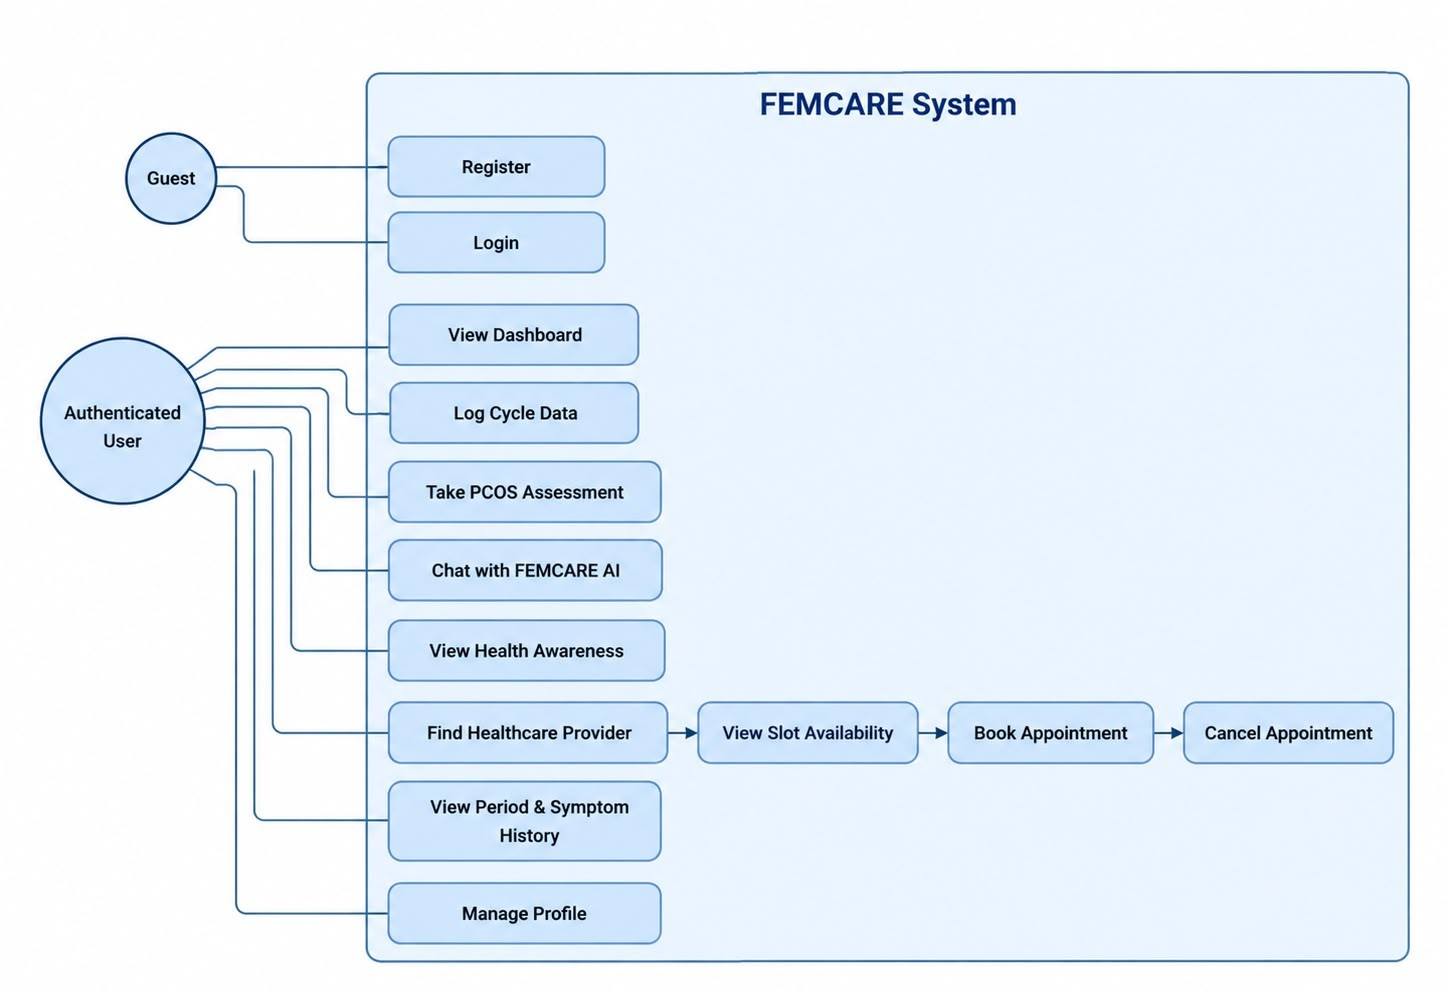
\includegraphics[width=0.85\textwidth]{3.1.jpeg}
\caption{Use Case Diagram of FEMCARE}
\label{fig:usecase}
\end{figure}

\begin{table}[h!]
\centering
\caption{Use Case Summary}
\label{tab:usecases}
\renewcommand{\arraystretch}{1.4}
\begin{tabular}{|p{1.2cm}|p{4cm}|p{2cm}|p{5.5cm}|}
\hline
\rowcolor[HTML]{D9D9D9}
\textbf{UC-ID} & \textbf{Use Case} & \textbf{Actor} & \textbf{Brief Description} \\
\hline
UC-01 & Register & Guest & Create a new account with personal and cycle details. \\
\hline
UC-02 & Login / Logout & Guest / User & Authenticate and manage the user session. \\
\hline
UC-03 & Log Daily Cycle & Auth. User & Record flow, pain, mood, and symptoms for a date. \\
\hline
UC-04 & View Dashboard & Auth. User & View cycle phase, latest logged data, and calendar. \\
\hline
UC-05 & Complete PCOS Assessment & Auth. User & Complete the 18-question quiz and view risk result. \\
\hline
UC-06 & Use AI Health Assistant & Auth. User & Ask reproductive health questions and receive scoped guidance. \\
\hline
UC-07 & Find Healthcare Provider & Auth. User & View providers on the map and in the list. \\
\hline
UC-08 & Book Appointment & Auth. User & Select a provider, date, and slot and confirm booking. \\
\hline
UC-09 & Cancel Appointment & Auth. User & Cancel a confirmed booking. \\
\hline
UC-10 & View Awareness Content & Auth. User & Browse, search, and filter health condition information. \\
\hline
UC-11 & View History & Auth. User & View period and symptom history records. \\
\hline
UC-12 & Update Profile & Auth. User & Edit name, email, cycle length, and last period date. \\
\hline
\end{tabular}
\end{table}

% ------------------------------------------------------------
\section{Feasibility Analysis}
\label{sec:feasibility}

\subsection{Technical Feasibility}

All technologies selected for FEMCARE are mature, actively maintained, and freely available for development use. React and FastAPI are widely adopted frameworks with extensive documentation. Supabase provides managed PostgreSQL with built-in authentication and Row Level Security, removing the need to implement authentication infrastructure from scratch. The Groq API provides low-latency LLM inference, and the Resend API provides a straightforward transactional email service. \cite{maity2025} The XGBoost library is a well-established gradient boosting implementation supported by scikit-learn's pipeline tooling. \cite{ahmed2023}\cite{zad2024} The combination of these services makes the proposed system technically feasible within the scope of a final year project.

\subsection{Operational Feasibility}

The application is a browser-based single-page application requiring no installation. Users interact with familiar interface patterns -- forms, toggles, cards, and maps -- that are consistent with standard web application conventions. The workflow from registration through cycle logging to assessment and booking follows a linear, task-oriented structure that is practical for the intended user group.

\subsection{Economic Feasibility}

The project makes use of free tiers of all external services: Supabase (free tier with 500 MB database and 50,000 monthly active users), Groq API (free tier with generous rate limits for development), and Resend (free tier with 3,000 emails per month). The frontend and backend are developed using open-source frameworks with no licensing costs. The project is therefore economically feasible for development and demonstration purposes at no cost beyond internet access and computing hardware.

% ------------------------------------------------------------



% ============================================================
% CHAPTER 4 -- SYSTEM DESIGN
% FEMCARE: An AI-Powered Women's Reproductive Health Platform
% ============================================================

\chapter{System Design}\doublespacing
\label{chap:design}

% ------------------------------------------------------------
\section{Introduction}
\label{sec:design-intro}

This chapter describes the design of the FEMCARE system: how its components are structured, how they interact, how data is organised in the database, and how the key workflows are realised. The requirements established in Chapter 3 are the basis for the design decisions described here. Implementation details, source-code-level logic, and testing are addressed in subsequent chapters.

% ------------------------------------------------------------
\section{System Architecture}
\label{sec:architecture}

FEMCARE follows a three-tier client--server architecture comprising a presentation tier, a logic tier, and a data tier, supplemented by three external cloud services.

\begin{itemize}
    \item \textbf{Presentation Tier} -- A React single-page application (SPA) built with Vite. The frontend handles all user interaction, client-side routing via React Router DOM, and communicates with the backend and database through HTTP and the Supabase JavaScript client.

    \item \textbf{Logic Tier} -- A Python FastAPI backend served by Uvicorn. This tier handles ML inference, AI chatbot requests, appointment booking operations, and administrative tasks such as email auto-confirmation. It is the only tier that holds service-role credentials and API keys.

    \item \textbf{Data Tier} -- A Supabase-managed PostgreSQL database that stores all user health data. Supabase Authentication manages user identity and JWT issuance. Row Level Security (RLS) policies enforce per-user data isolation at the database level.

    \item \textbf{External Services} -- Three cloud services are integrated: the Groq API provides LLM inference for the AI health assistant; the Resend API delivers transactional appointment emails; and OpenStreetMap tiles (rendered via Leaflet) provide the interactive provider map.
\end{itemize}

The communication paths between tiers are shown in Table~\ref{tab:arch-comms}. Figure~\ref{fig:architecture} shows the overall system architecture of FEMCARE.

\begin{figure}[h!]
\centering
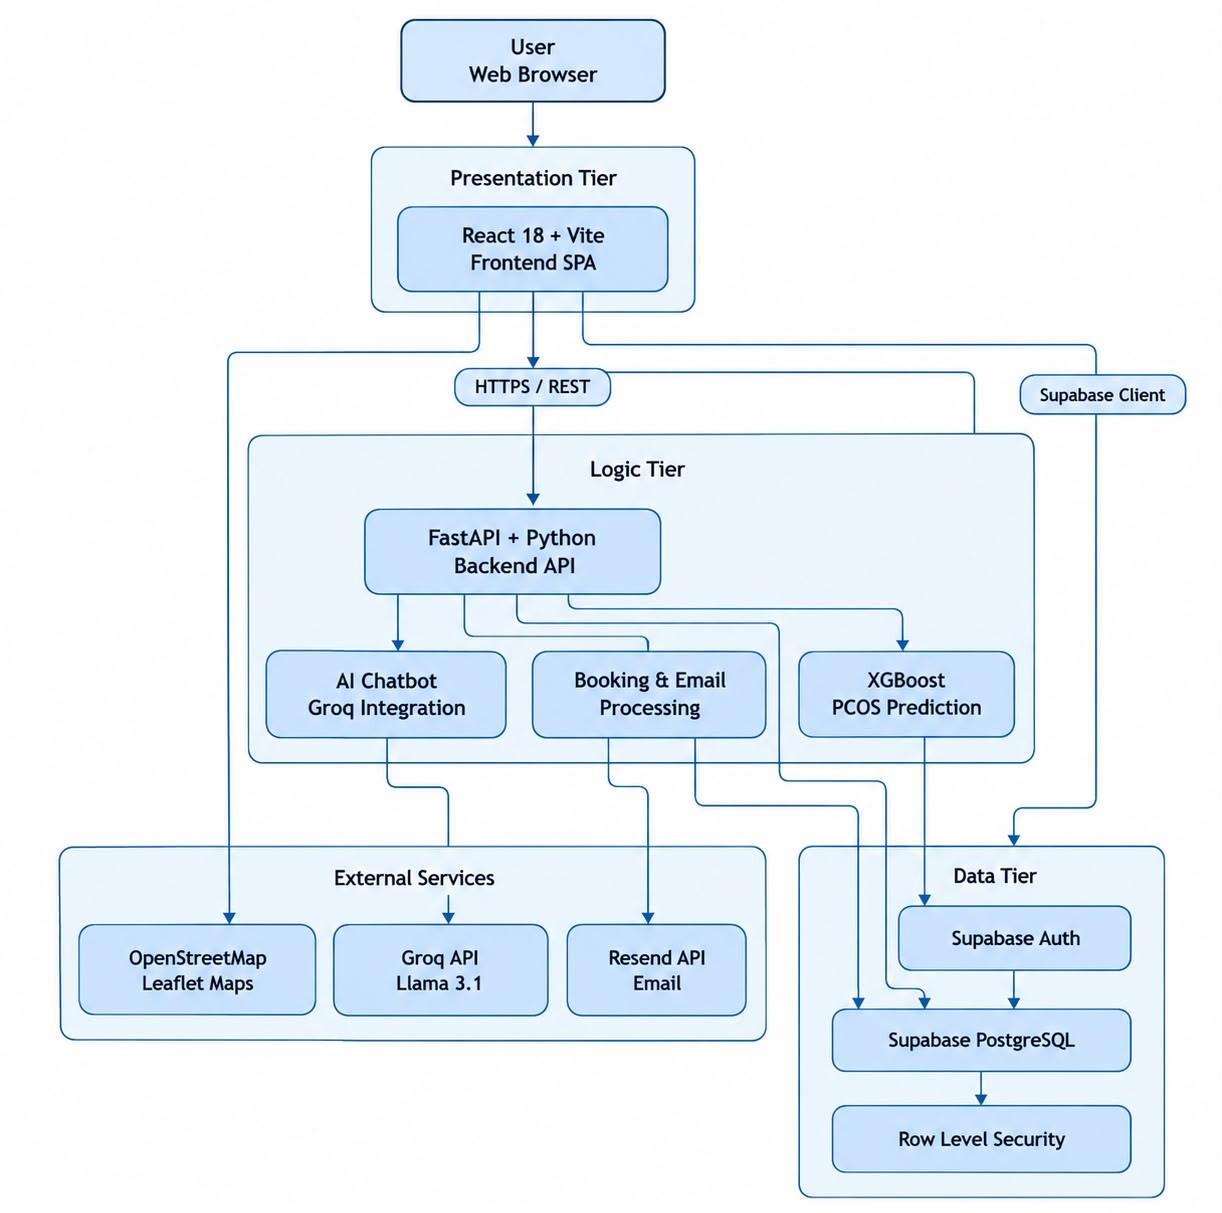
\includegraphics[width=0.90\textwidth]{4.1.jpeg}
\caption{System Architecture of FEMCARE}
\label{fig:architecture}
\end{figure}

\begin{table}[h!]
\centering
\caption{Inter-Tier Communication}
\label{tab:arch-comms}
\renewcommand{\arraystretch}{1.4}
\begin{tabular}{|p{3.2cm}|p{3.2cm}|p{3cm}|p{3cm}|}
\hline
\rowcolor[HTML]{D9D9D9}
\textbf{From} & \textbf{To} & \textbf{Protocol} & \textbf{Credential} \\
\hline
React Frontend & Supabase DB & HTTPS (supabase-js) & Anon key + JWT \\
\hline
React Frontend & FastAPI Backend & HTTPS REST (fetch) & Bearer JWT (optional) \\
\hline
FastAPI Backend & Supabase DB & HTTPS (supabase-py) & Service role key \\
\hline
FastAPI Backend & Groq API & HTTPS & GROQ\_API\_KEY \\
\hline
FastAPI Backend & Resend API & HTTPS (httpx) & RESEND\_API\_KEY \\
\hline
\end{tabular}
\end{table}

A key architectural decision is the dual access path to Supabase. The frontend queries Supabase directly for cycle data, period records, and symptom history using the anon key; RLS policies automatically restrict these queries to the authenticated user's own rows. The backend uses the service role key, which bypasses RLS, only for operations that require elevated access -- specifically booking management and email confirmation -- where server-side identity verification has already been performed.

% ------------------------------------------------------------
\section{Module Design}
\label{sec:modules}

FEMCARE is organised into eight functional modules. Table~\ref{tab:modules} summarises each module and its primary responsibility.

\begin{table}[h!]
\centering
\caption{FEMCARE Module Summary}
\label{tab:modules}
\renewcommand{\arraystretch}{1.4}
\begin{tabular}{|p{3.8cm}|p{3.5cm}|p{5.5cm}|}
\hline
\rowcolor[HTML]{D9D9D9}
\textbf{Module} & \textbf{Primary Files} & \textbf{Responsibility} \\
\hline
Authentication & AuthContext.jsx & Registration, login, session management, profile loading \\
\hline
Cycle Tracking & LogCycle.jsx, cycleService.js, symptomService.js & Daily logging of flow, pain, mood, and symptoms \\
\hline
Dashboard & Dashboard.jsx & Real-time cycle phase, health summary, compact chatbot \\
\hline
PCOS Assessment & HealthAssessment.jsx, main.py (/api/predict) & 18-feature quiz, ML prediction, result display \\
\hline
AI Health Assistant & ChatBot.jsx, femcare\_chatbot.py & Scoped LLM chatbot with user-context enrichment \\
\hline
Find Care \& Booking & FindCare.jsx, main.py (/api/book-appointment) & Provider map, slot selection, booking, cancellation \\
\hline
Health Awareness & Awareness.jsx, awarenessData.js & Condition content, warning signs, prevention habits \\
\hline
Email Notification & femcare\_email.py & Confirmation and cancellation emails via Resend API \\
\hline
\end{tabular}
\end{table}

% ------------------------------------------------------------
\section{Data Flow for Key Workflows}
\label{sec:dataflow}

\subsection{User Authentication and Profile Creation}
\label{subsec:flow-auth}

When a new user registers, the frontend submits credentials and profile metadata to Supabase Authentication. If email confirmation is required, the backend's \texttt{/api/confirm-email} endpoint confirms the account using the Supabase Admin API. Upon successful authentication, a PostgreSQL trigger (\texttt{handle\_new\_user}) fires automatically and inserts a corresponding row into the \texttt{public.users} table, copying the name, age, and cycle configuration from the authentication metadata. On subsequent logins, the \texttt{AuthContext} component queries \texttt{public.users} directly to load the full profile.

\subsection{Cycle Logging and Dashboard Synchronisation}
\label{subsec:flow-cycle}

When a user saves a daily log, the \texttt{LogCycle} page upserts a row into the \texttt{cycle\_logs} table with a unique constraint on \texttt{(user\_id, log\_date)}. Simultaneously, the \texttt{syncSymptomsForDate} function deletes any existing symptom rows for that date and inserts fresh rows into the \texttt{symptoms} table, applying a name-mapping layer to reconcile display names with the database's CHECK constraint values. The Dashboard queries \texttt{getLatestCycleLog()} and \texttt{getRecentSymptoms()} on load to reflect the most recent logged data in real time.

\subsection{PCOS Assessment}
\label{subsec:flow-pcos}

The user completes the 18-step assessment wizard. Where both LH and FSH values are entered, the frontend automatically calculates the \texttt{LH\_FSH\_ratio} field. On submission, the frontend POSTs the 18 feature values to \texttt{/api/predict} with a Bearer token. The backend authenticates the request, stores the raw inputs in \texttt{health\_assessments}, runs the XGBoost pipeline, stores the result in \texttt{assessment\_results}, and returns the risk classification and confidence to the frontend. If the model is unavailable, the heuristic fallback is used and the same response structure is returned.

\subsection{AI Health Assistant}
\label{subsec:flow-chat}

A user message is sent to \texttt{/api/chat}. The backend performs a two-stage scope check: first a keyword-based Python filter, then the LLM system prompt acts as a second restriction layer. If the query is within scope, the backend optionally enriches the context with the user's last period date and recent symptoms from Supabase, then calls the Groq API. The reply is returned to the frontend and rendered in the chat interface.

\subsection{Appointment Booking}
\label{subsec:flow-booking}

The user selects a provider, date, and time slot, then confirms the booking. The frontend sends the selection to \texttt{/api/book-appointment} with a Bearer token. The backend resolves the user's name from \texttt{public.users}, inserts a row into the \texttt{bookings} table, and -- if the insert succeeds -- calls the email service. A partial unique index on \texttt{(provider\_id, appointment\_date, appointment\_slot)} filtered by \texttt{status = 'confirmed'} prevents double-booking at the database level, returning HTTP 409 on violation. The sequence diagram for this workflow is shown in Figure~\ref{fig:booking-sequence}.

\begin{figure}[h!]
\centering
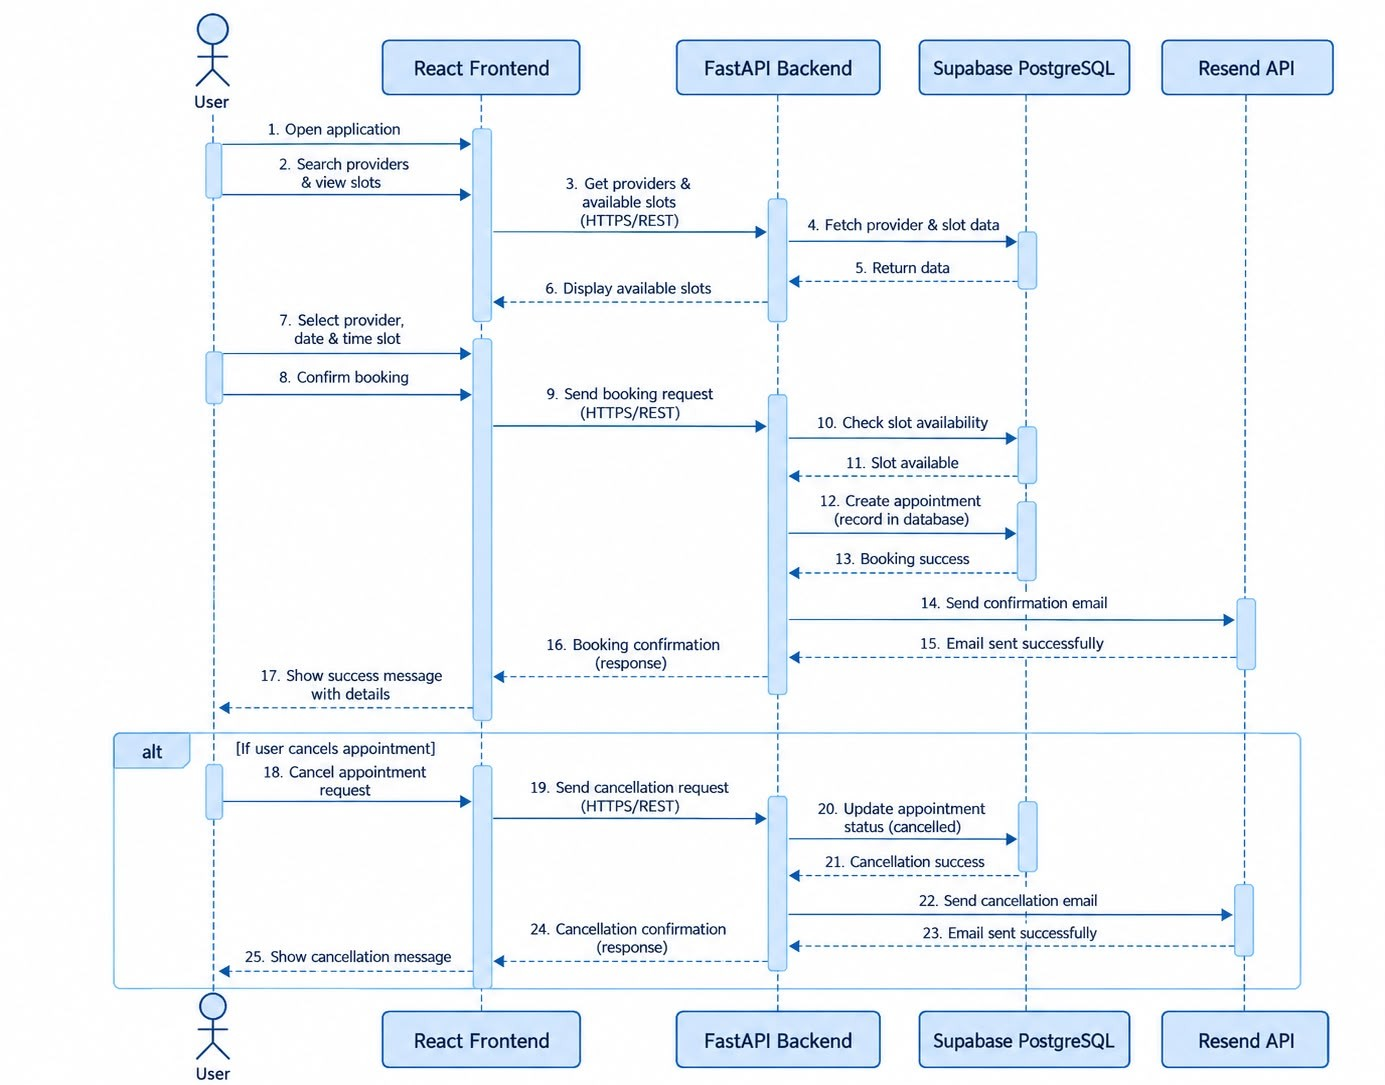
\includegraphics[width=0.88\textwidth]{4.2.jpeg}
\caption{Appointment Booking Sequence Diagram}
\label{fig:booking-sequence}
\end{figure}

% ------------------------------------------------------------
\section{Database Design}
\label{sec:database}

\subsection{Entity Relationships}
\label{subsec:er}

The database contains eight tables linked by foreign key relationships. The central entity is \texttt{public.users}, which extends Supabase's \texttt{auth.users} table. All other user data tables reference \texttt{users} with cascade deletion. The relationships are described in Table~\ref{tab:er}. Figure~\ref{fig:er} presents the entity-relationship diagram.

\begin{figure}[h!]
\centering
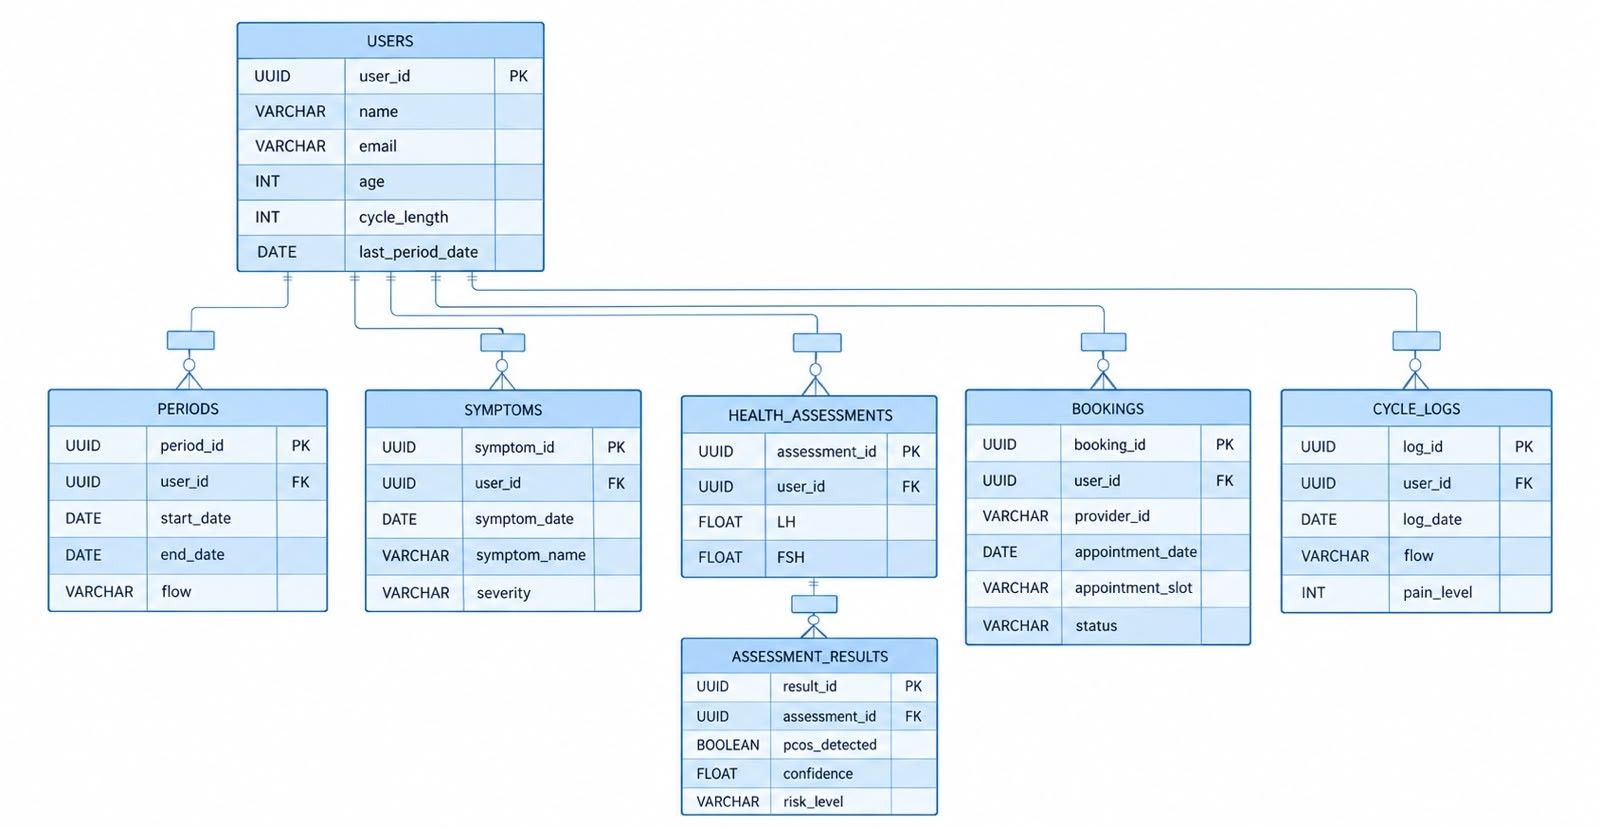
\includegraphics[width=0.88\textwidth]{4.3.jpeg}
\caption{Entity-Relationship Diagram of FEMCARE}
\label{fig:er}
\end{figure}

\begin{table}[h!]
\centering
\caption{Table Relationships}
\label{tab:er}
\renewcommand{\arraystretch}{1.4}
\begin{tabular}{|p{3.5cm}|p{2.5cm}|p{6.5cm}|}
\hline
\rowcolor[HTML]{D9D9D9}
\textbf{Table} & \textbf{Relationship} & \textbf{Notes} \\
\hline
auth.users $\rightarrow$ users & 1:1 & Trigger auto-creates profile on signup \\
\hline
users $\rightarrow$ cycle\_logs & 1:N & Unique per (user\_id, log\_date) \\
\hline
users $\rightarrow$ periods & 1:N & Unique per (user\_id, start\_date) \\
\hline
users $\rightarrow$ symptoms & 1:N & Keyed by (user\_id, symptom\_date) \\
\hline
periods $\rightarrow$ cycle\_history & 1:1 & Auto-populated by trigger \\
\hline
users $\rightarrow$ health\_assessments & 1:N & Stores raw ML input features \\
\hline
health\_assessments $\rightarrow$ assessment\_results & 1:1 & Stores ML prediction output; immutable \\
\hline
users $\rightarrow$ bookings & 1:N & Partial unique index on confirmed slots \\
\hline
\end{tabular}
\end{table}

\subsection{Key Table Design Decisions}
\label{subsec:table-design}

Several design decisions in the schema are worth noting at this level:

\begin{itemize}
    \item \textbf{cycle\_logs} stores \texttt{symptoms} and \texttt{moods} as PostgreSQL text arrays, reflecting the multi-select nature of the logging interface. The \texttt{symptoms} table stores the same data in a normalised, one-row-per-symptom form to support per-symptom queries on the Dashboard.

    \item \textbf{health\_assessments} column names match the feature names in the serialised XGBoost model file exactly. This ensures that the DataFrame constructed in the backend aligns with the model without any column remapping.

    \item \textbf{assessment\_results} has no UPDATE or DELETE RLS policy, making assessment history immutable by design.

    \item \textbf{cycle\_history} is populated automatically by a PostgreSQL trigger (\texttt{calculate\_cycle\_metrics}) that fires after an insert or update on \texttt{periods}, computing cycle length as the interval between consecutive period start dates.

    \item \textbf{bookings} uses a partial unique index rather than a table-level constraint so that the same slot can be re-booked after cancellation, since cancelled rows are excluded from the uniqueness check.
\end{itemize}

\subsection{Row Level Security}
\label{subsec:rls}

Every user data table has RLS enabled. All SELECT, INSERT, UPDATE, and DELETE policies are conditioned on \texttt{auth.uid() = user\_id}, ensuring that Supabase client queries from the frontend are automatically scoped to the authenticated user without relying on application-layer filtering. Assessment results have SELECT-only RLS; they cannot be modified or deleted through the client.

% ------------------------------------------------------------
\section{AI and ML Component Design}
\label{sec:ai-design}

\subsection{PCOS Assessment Pipeline}
\label{subsec:pcos-design}

The PCOS assessment is designed as a two-stage pipeline. In the first stage, the frontend collects 18 feature values through a guided wizard and derives the LH/FSH ratio automatically. In the second stage, the backend loads the serialised XGBoost pipeline (\texttt{cycle\_prediction\_xgboost\_pipeline.pkl}) and a feature-name list (\texttt{pcos\_features.pkl}) at application startup. At inference time, the input values are assembled into a pandas DataFrame, columns are aligned to the model's expected feature order using the loaded feature list, and the model's \texttt{predict} and \texttt{predict\_proba} methods produce the binary classification and confidence score. The risk level (Low, Moderate, or High Risk) is derived from the predicted class and confidence. A heuristic scoring function counts clinically relevant PCOS markers and serves as the fallback when the model cannot be loaded. Figure~\ref{fig:pcos-assessment} illustrates this assessment workflow.

\begin{figure}[h!]
\centering
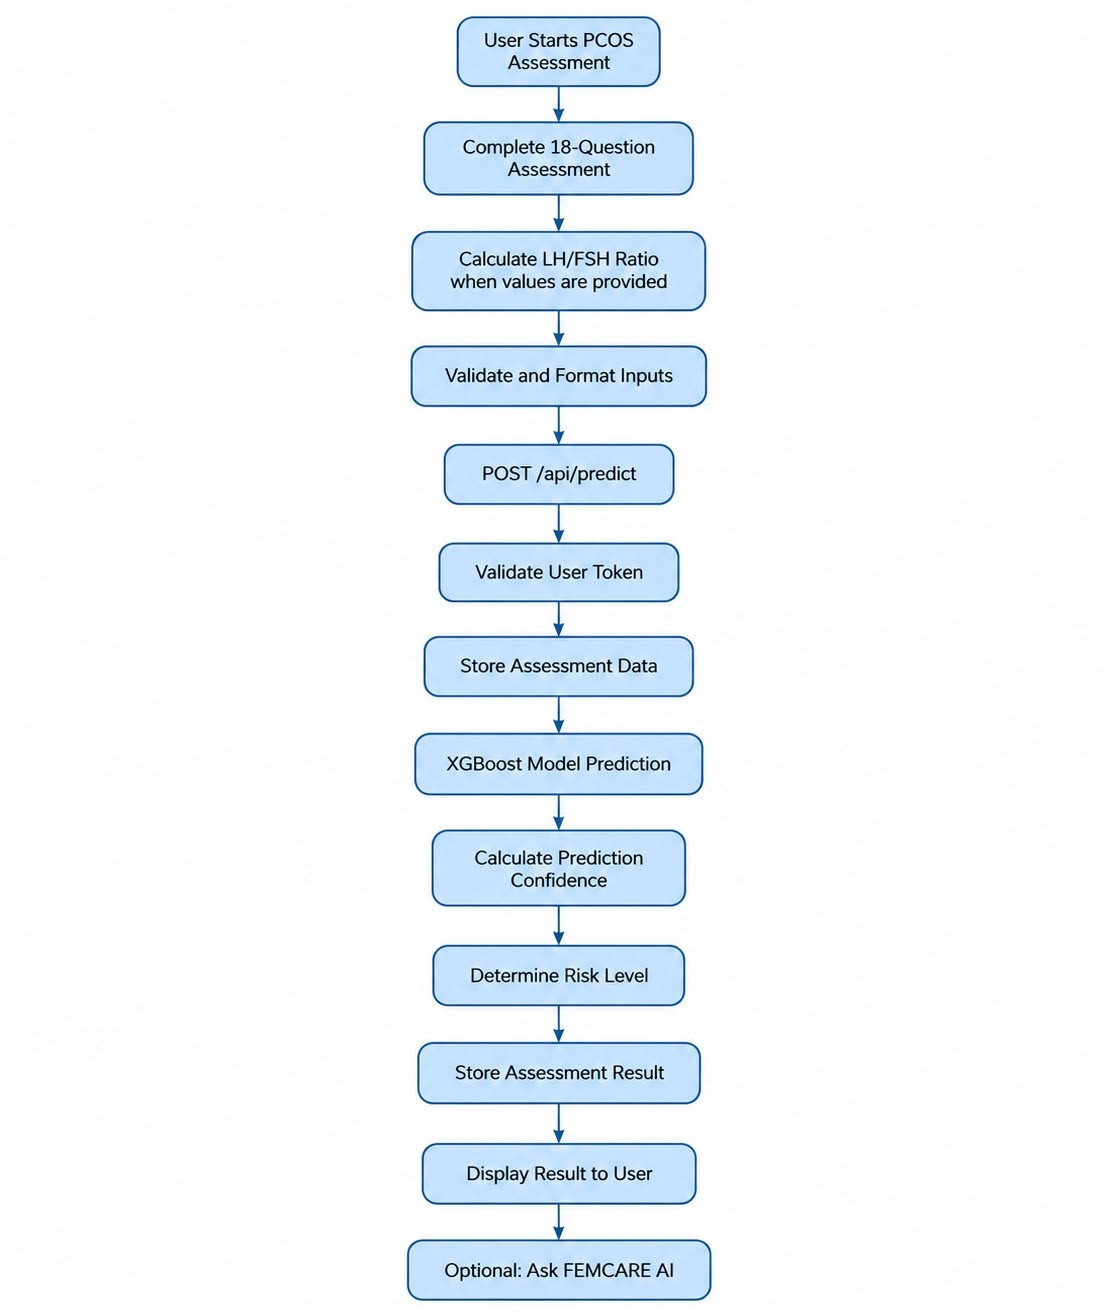
\includegraphics[width=0.25\textwidth]{4.4.jpeg}
\caption{PCOS Assessment Workflow}
\label{fig:pcos-assessment}
\end{figure}

\subsection{AI Health Assistant Pipeline}
\label{subsec:chat-design}

The chatbot is implemented as a sequential pipeline in \texttt{femcare\_chatbot.py}. The pipeline has five stages:

\begin{enumerate}
    \item \textbf{Scope check} -- A keyword-based filter tests the message against a set of out-of-scope categories (programming, sports, weather, entertainment). If any health-related keyword is also present, the message is considered in scope regardless of other matches.
    \item \textbf{Urgency check} -- If urgency keywords are detected (e.g. severe pain, fainting), an urgency instruction is appended to the system prompt.
    \item \textbf{Knowledge retrieval} -- A topic is detected from the message and the corresponding entry from the structured knowledge base is formatted as context.
    \item \textbf{User context enrichment} -- If the user is authenticated, their last period date and recent symptoms are fetched from Supabase and appended to the user turn.
    \item \textbf{LLM call} -- The Groq API is called with the FEMCARE system prompt and the assembled user content. Temperature is set to 0.4 and \texttt{max\_tokens} to 400 to produce concise, medically cautious responses. \cite{maity2025}
\end{enumerate}

% ------------------------------------------------------------
\section{Security Design}
\label{sec:security-design}

The security design of FEMCARE operates at three levels:

\textbf{Authentication.} User identity is managed by Supabase Authentication. The platform issues short-lived JWTs that are automatically refreshed by the client. Passwords are stored and verified exclusively within Supabase's authentication service and are never accessible to the application layer.

\textbf{Authorisation and data isolation.} As described in Section~\ref{subsec:rls}, RLS policies enforce per-user data access at the database level. The backend validates the Bearer token on every protected endpoint by calling \texttt{supabase.auth.get\_user(token)} before any database operation. This ensures that a user cannot access or modify another user's bookings, assessments, or health logs even if they possess a valid JWT.

\textbf{Credential management.} All service credentials -- the Supabase service role key, GROQ\_API\_KEY, and RESEND\_API\_KEY -- are stored in a server-side \texttt{.env} file and loaded at runtime via \texttt{python-dotenv}. \cite{kotz2016}

% ------------------------------------------------------------


% ============================================================
% CHAPTER 5 -- METHODOLOGY (SYSTEM IMPLEMENTATION)
% FEMCARE: An AI-Powered Women's Reproductive Health Platform
% ============================================================

\chapter{Methodology}\doublespacing
\label{chap:implementation}

% ------------------------------------------------------------
\section{Introduction}
\label{sec:impl-intro}

This chapter presents the methodology adopted for the development of the FemCare system, an AI-driven platform for women’s reproductive health monitoring and risk awareness. The methodology describes the complete process followed for data preparation, preprocessing, feature construction, machine learning model development, model evaluation, prediction generation, and integration of the trained models with the application.

The machine learning component of FemCare consists of two independent prediction tasks. The first task is a binary classification problem for assessing the risk of PMOS, for which an XGBoost classifier is employed. The second task is a regression problem for predicting the length of the user's next menstrual cycle, for which an XGBoost regressor is used. Both models are trained separately because they have different target variables and prediction objectives.

The overall methodology follows the sequence:

Dataset Collection $\rightarrow$ Data Inspection $\rightarrow$ Data Preprocessing $\rightarrow$ Feature Preparation $\rightarrow$ Data Splitting $\rightarrow$ XGBoost Model Training $\rightarrow$ Prediction $\rightarrow$ Performance Evaluation $\rightarrow$ Model Saving $\rightarrow$ Application Integration

The PMOS model uses pmos as its target variable, while the menstrual-cycle model uses Next\_Cycle\_Length as its target variable. The trained models are subsequently incorporated into the FemCare backend to generate predictions from user-provided information.

% ------------------------------------------------------------
\section{Overall System Approach}
\label{system approach}
The FemCare system follows a data-driven and modular approach in which user information is processed through dedicated prediction pipelines. The methodology separates the PMOS risk-assessment task from the menstrual-cycle prediction task so that each model can be developed, evaluated, and deployed according to the requirements of its respective prediction problem.

The overall system methodology consists of the following major stages:

\begin{itemize}
    \item \textbf{Data Collection:} Relevant reproductive-health and menstrual-cycle datasets are prepared for model development.
    \item \textbf{Data Inspection:} The datasets are examined for their dimensions, data types, target distributions, missing values, and feature characteristics.
    \item \textbf{Data Pre-processing:} Unnecessary attributes are removed, input variables are converted into suitable numerical or categorical representations, and missing values are handled.
    \item \textbf{Feature Preparation:}  Relevant physiological, menstrual, symptom, temporal, and historical-cycle attributes are prepared for model training.
    \item \textbf{Data Splitting:} Appropriate training and testing strategies are applied. Stratified splitting is used for PCOS classification, while user-level splitting is used for menstrual-cycle prediction.
    \item \textbf{Model Development:} XGBoost models are trained independently for classification and regression.
    \item \textbf{Prediction:} The trained models generate PCOS class and probability predictions or next-cycle length predictions.
    \item \textbf{Evaluation:} Appropriate classification and regression metrics are calculated to assess model performance.
    \item \textbf{Model Serialization:} The trained models and required pre-processing components are saved for application deployment.
    \item \textbf{Application Integration:} The saved models are connected to the FastAPI backend and accessed by the FemCare frontend through REST APIs. 
\end{itemize}
This approach ensures that the same preprocessing and feature arrangement used during model development can be maintained when new user data is processed by the deployed application.

\section{Data Preprocessing}
\label{sec:datapre}
The machine learning component of FemCare uses separate datasets for PCOS risk assessment and menstrual-cycle prediction.

\subsection{PMOS Dataset}
The PMOS prediction experiment uses a dataset containing 10,000 records and 48 columns. The dataset contains reproductive-health-related variables covering menstrual, hormonal, physical-health, and other relevant characteristics. The dataset was prepared using information derived from clinical literature and a feature set based on Kerala clinical data. The data used for experimentation is organized in the Final\_Dataset worksheet.

The target variable for the classification task is PMOS. The value of this variable represents the binary class to be predicted by the XGBoost classifier.

Before model training, the dataset was inspected to determine:
\begin{itemize}
    \item Number of observations
    \item Number of variables
    \item Feature names
    \item Data types
    \item Missing-value distribution
    \item Target-variable distribution
\end{itemize}
The following attributes were excluded from the input feature matrix:
\begin{itemize}
    \item patient\_id
    \item blood\_group\_label
    \item cycle\_regularity\_label
    \item bmi\_category
    \item age\_group
    \item PMOS
\end{itemize}
he pmos attribute was excluded from the input features because it represents the prediction target.

Therefore, if $D$ represents the original PMOS dataset, the input feature matrix can be represented as:
\begin{equation}
X = D - \{ \text{patient\_id}, \text{blood\_group\_label}, \text{cycle\_regularity\_label}, \text{bmi\_category}, \text{age\_group}, \text{pcos} \}
\end{equation}
and the target vector is:
$y = \text{pcos}$

The project methodology documentation confirms that the PCOS dataset contains 10,000 records and 48 columns and that the pcos attribute is used as the classification target.

\subsection{Menstrual-Cycle Dataset}
A separate longitudinal menstrual-cycle dataset is used for next-cycle prediction. The dataset contains menstrual records organized on a per-user basis. Each record contains information related to an individual's menstrual history, cycle characteristics, symptoms, and temporal information.

The cycle dataset includes attributes such as:
\begin{itemize}
    \item User ID
    \item Cycle Number
    \item Period Start Date
    \item Period End Date
    \item Cycle Length
    \item Period Duration
    \item Flow
    \item Cramps
    \item Headache
    \item Bloating
\end{itemize}
Additional historical cycle features are constructed from previous menstrual cycles.

The target variable is Next\_Cycle\_Length, which represents the length of the following menstrual cycle. The target is generated by arranging the records chronologically for each user and shifting the current cycle length by one period.

Thus:
\begin{equation}
\text{NextCycleLength}_{t} = \text{CycleLength}_{t+1}
\end{equation}
Records for which the current or future cycle length is unavailable or invalid are excluded from the modeling dataset.

\section{Data Pre-Processing}
\label{sec:dataPre}
Data preprocessing is performed before model training to ensure that the input data is consistent, valid, and compatible with the machine learning algorithms.

\subsubsection{PCOS Data Pre-Processing}
For the PCOS model, unnecessary identifiers and redundant categorical-label columns are removed before training. The remaining input features are converted into numerical form.

Each feature is processed using numerical conversion. If a value cannot be converted into a valid numerical representation, it is treated as a missing value.

Although the original PCOS dataset used for experimentation contains no missing values, a median imputer is retained as part of the prediction pipeline. This ensures that missing values originating from future user input can be handled consistently during application-level prediction.

The median-imputation process can be represented as:
\begin{equation}
x'_i = 
\begin{cases} 
x_i, & \text{if } x_i \text{ is available} \\ 
\text{median}(X_j), & \text{if } x_i \text{ is missing} 
\end{cases}
\end{equation}
where $X_j$ represents the corresponding feature.

After preprocessing, the dataset is divided into training and testing subsets using an 80:20 ratio. A fixed random state of 42 is used to maintain reproducibility, and stratification based on the PCOS target is applied to preserve the class distribution in the two subsets. The resulting test set contains 2,000 records, consisting of 1,340 No-PCOS cases and 660 PCOS cases.

\subsubsection{Menstrual-Cycle Data Preprocessing}

The menstrual-cycle dataset requires additional temporal preprocessing because the prediction task is based on sequential menstrual records.

First, records are organized according to User\_ID and Period\_Start\_Date so that each user's menstrual history is maintained in chronological order. The next-cycle target is then created by shifting the cycle length forward by one record within each user group.

Historical features are also generated using the previous three cycle lengths:
\[
\text{PreviousCycle}_1, \quad \text{PreviousCycle}_2, \quad \text{PreviousCycle}_3
\]

The average of the available previous cycles is calculated as:
\begin{equation}
    \text{PreviousCycleAverage} = \frac{C_1 + C_2 + C_3}{3}
\end{equation}

when all three values are available.
The standard deviation of previous cycle lengths is also calculated to represent recent cycle-length variability.

For numerical variables, missing values are handled using median imputation. For categorical variables, missing values are replaced using the most frequent category, after which categorical variables are transformed using one-hot encoding. Unknown categories encountered during prediction are ignored so that new user inputs do not cause preprocessing failures.

A GroupShuffleSplit strategy is used with User\_ID as the grouping variable. The test size is 20\% and the random state is 42. Consequently, records belonging to the same user are retained within a single partition rather than being distributed between training and testing sets. This is important for longitudinal data because it reduces the possibility of the same user's historical records appearing in both training and testing data.


\section{Feature Selection}
\label{sec:featselec}

Feature selection is performed separately for the PCOS classification and menstrual-cycle prediction models.

For PCOS prediction, identifier and redundant categorical-label attributes such as patient\_id, blood\_group\_label, cycle\_regularity\_label, bmi\_category, and age\_group are excluded. The remaining health-related variables are used as input features. XGBoost feature-importance analysis is then used to identify the variables contributing most to the model predictions. The most important features include follicle number on the right, total follicle count, follicle number on the left, blood glucose, cycle regularity, AMH, LH, and the LH/FSH ratio. \cite{zad2024} These importance values represent model-level contribution and do not indicate causality.

For menstrual-cycle prediction, the features include current cycle information, symptoms, temporal attributes, and historical cycle information. Three previous cycle lengths, their average, and standard deviation are included to capture recent cycle patterns and variability. Date-related features such as start month, start day, and start weekday are also derived from the period start date.

\section{Machine Learning Model}
\label{sec:MLmodel}
FemCare uses two independent XGBoost models for its prediction tasks. An XGBClassifier is used for PCOS risk classification, while an XGBRegressor is used for menstrual-cycle length prediction.

The PCOS model predicts a binary output using pcos as the target variable, whereas the cycle model predicts the continuous Next\_Cycle\_Length value. Both models are trained independently because the two tasks require different prediction objectives and evaluation procedures.

\subsection{XGBoost Algorithm}
XGBoost (Extreme Gradient Boosting) is an ensemble learning algorithm based on decision trees. It builds trees sequentially, with each new tree attempting to reduce the errors made by the previous trees. \cite{ahmed2023}

For PMOS classification, the model uses the following configuration:

\renewcommand{\arraystretch}{1.4} % Adds clean padding to rows
\begin{table}[h]
\centering
\begin{tabular}{|l|r|}
\hline
\textbf{Parameter} & \textbf{Value} \\ \hline
Number of estimators & 500 \\ \hline
Maximum depth & 5 \\ \hline
Learning rate & 0.03 \\ \hline
Subsample & 0.85 \\ \hline
Column sample by tree & 0.85 \\ \hline
Minimum child weight & 1 \\ \hline
Objective & \texttt{binary:logistic} \\ \hline
Evaluation metric & \texttt{logloss} \\ \hline
Random state & 42 \\ \hline
\end{tabular}
\caption{XGBoost Model Hyperparameters}
\label{tab:hyperparameters}
\end{table}

For menstrual-cycle prediction, the XGBoost regressor uses 500 estimators, a maximum depth of 5, a learning rate of 0.03, 0.85 subsampling, 0.85 feature sampling, and reg:squarederror as the regression objective.

The PCOS classifier produces both a predicted class and its corresponding prediction probability, while the regression model produces the estimated length of the next menstrual cycle.

\section{Evaluation Metrics}
Different evaluation metrics are used for the two prediction tasks.

\textbf{PCOS Classification}
The PCOS model is evaluated using:
\begin{itemize}
    \item Accuracy
    \item Precision
    \item Recall
    \item F1-score
    \item ROC-AUC
    \item Confusion Matrix
    \item Five-fold Stratified Cross-Validation
\end{itemize}

The final PCOS model achieved 99.85\% accuracy, 99.85\% precision, 99.70\% recall, 99.77\% F1-score, and 1.0000 ROC-AUC. The five-fold cross-validation accuracy was 99.93\% ± 0.07\%.

\textbf{Menstrual-Cycle Prediction}

The cycle prediction model is evaluated using:
\begin{itemize}
    \item Mean Absolute Error (MAE)
    \item Root Mean Squared Error (RMSE)
$R^2$
    \item Prediction accuracy within ±2 days
\end{itemize}

The final model achieved an MAE of 1.89 days, RMSE of 2.29 days, $R^2$ of 0.5274, and 57.68\% of predictions within ±2 days.


% ------------------------------------------------------------
\section{Advantages of Methodology}
\label{sec:AdvMetho}
The methodology provides the following advantages:
\begin{itemize}
    \item \textbf{Separate prediction models:} Classification and regression tasks are handled independently.
    \item \textbf{Reproducibility:}Fixed random states are used during data splitting..
    \item \textbf{Appropriate data splitting:}Stratification is used for PCOS classification, while user-level splitting is used for cycle prediction.
    \item \textbf{Consistent preprocessing:}The same preprocessing components are reused during deployment.
    \item \textbf{Feature analysis:}XGBoost feature importance provides information about influential input variables.
    \item \textbf{Task-specific evaluation:}Different metrics are used according to the prediction problem.
    \item \textbf{Application integration:}The trained models are directly integrated with the FastAPI backend.
\end{itemize}

\section{Limitations}
The methodology has the following limitations:
\begin{itemize}
    \item Model performance depends on the datasets used for training and evaluation.
    \item External validation using independent datasets is still required.
    \item Prediction quality depends on the accuracy and completeness of user-provided information.
    \item Menstrual-cycle length naturally varies between individuals and between cycles.
    \item Feature-importance values represent model contribution and should not be interpreted as causal medical relationships.
    \item The current system requires further clinical validation before potential clinical deployment. \cite{pi2025}
    \item Privacy and security must be carefully maintained because the system handles sensitive reproductive-health information. \cite{kotz2016}
\end{itemize}


\section{Conclusion}
\label{sec:Concl}
The methodology of FemCare provides a structured machine learning pipeline covering data preparation, preprocessing, feature selection, model training, evaluation, and application integration. Two XGBoost models are used: an XGBoost classifier for PCOS risk assessment and an XGBoost regressor for menstrual-cycle length prediction.

The PCOS model uses stratified classification methodology, while the cycle model incorporates historical menstrual information and user-level data separation. The trained models are integrated with the FastAPI backend to generate predictions from new user inputs and present the results through the FemCare application.

Overall, the methodology provides the technical foundation for the FemCare system while recognizing the need for further external validation, clinical evaluation, and secure deployment.










% ============================================================
% CHAPTER 6 -- IMPLEMENTATION (TESTING AND RESULTS)
% FEMCARE: An AI-Powered Women's Reproductive Health Platform
% ============================================================

\chapter{Implementation}\doublespacing
\label{chap:testing}

% ------------------------------------------------------------
\section{Introduction}
\label{sec:test-intro}

This chapter presents the functional testing performed on FEMCARE and the results observed from the running system. Testing was conducted manually against the live application. The project repository also contains backend test scripts (\texttt{test\_backend.py}, \texttt{test\_double\_booking\_prevention.py}, \texttt{test\_security\_smoke.js}) used to verify specific API and database behaviours. Results are limited to behaviours directly observed from the implemented system; no accuracy metrics or performance benchmarks are claimed.

% ------------------------------------------------------------
\section{Functional Test Cases}
\label{sec:test-functional}

Test cases are organised by feature area. Each table uses the columns: Test ID, Action/Input, Expected Result, and Status.


\begin{table}[h!]
\centering
\caption{Authentication Test Cases}
\label{tab:tc-auth}
\renewcommand{\arraystretch}{1.3}
\setlength{\tabcolsep}{5pt}
\begin{tabular}{|p{1cm}|p{4.5cm}|p{5cm}|p{1.5cm}|}
\hline
\rowcolor[HTML]{D9D9D9}
\textbf{ID} & \textbf{Action / Input} & \textbf{Expected Result} & \textbf{Status} \\
\hline
TC-A1 & Register with valid name, email, password, age, cycle length & Account created; profile inserted in \texttt{public.users}; Dashboard loaded & Pass \\
\hline
TC-A2 & Register with an already-used email & Error displayed; no duplicate account & Pass \\
\hline
TC-A3 & Login with correct credentials & Session established; user's name shown on Dashboard & Pass \\
\hline
TC-A4 & Login with wrong password & Error shown; no session created & Pass \\
\hline
TC-A5 & Navigate to \texttt{/dashboard} without a session & Redirected to \texttt{/login} & Pass \\
\hline
TC-A6 & Update cycle length in Profile and save & New value persisted in \texttt{public.users} and reflected on reload & Pass \\
\hline
\end{tabular}
\end{table}

\subsection{Cycle Logging and Dashboard}
\label{subsec:tc-cycle}
\begin{figure}[H]
    \centering
    \includegraphics[width=0.9]\textwidth]{Dashboard.jpeg}
    \caption{Caption of the figure}
    \label{fig:Cycle Logging and Dashboard}
\end{figure}

\begin{table}[h!]
\centering
\caption{Cycle Logging and Dashboard Test Cases}
\label{tab:tc-cycle}
\renewcommand{\arraystretch}{1.3}
\setlength{\tabcolsep}{5pt}
\begin{tabular}{|p{1cm}|p{4.5cm}|p{5cm}|p{1.5cm}|}
\hline
\rowcolor[HTML]{D9D9D9}
\textbf{ID} & \textbf{Action / Input} & \textbf{Expected Result} & \textbf{Status} \\
\hline
TC-C1 & Log Heavy flow, Cramps, Fatigue for today & Data upserted to \texttt{cycle\_logs}; symptoms synced to \texttt{symptoms} table & Pass \\
\hline
TC-C2 & Open Dashboard after TC-C1 & Flow ``Heavy'', pills ``Cramps'' and ``Fatigue'' shown in Latest Log card & Pass \\
\hline
TC-C3 & Re-log same date with Light flow & Row updated; Dashboard shows ``Light'' & Pass \\
\hline
TC-C4 & Log ``Backache'' & Stored as ``Back Pain'' in \texttt{symptoms} (CHECK constraint satisfied) & Pass \\
\hline
TC-C5 & Reload browser after logging & Same data shown; confirms Supabase persistence & Pass \\
\hline
TC-C6 & New user with no logs & Dashboard shows empty-state message; no blank screen & Pass \\
\hline
\end{tabular}
\end{table}

\subsection{PCOS Assessment}
\label{subsec:tc-pcos}
\begin{figure}[H]
    \centering
    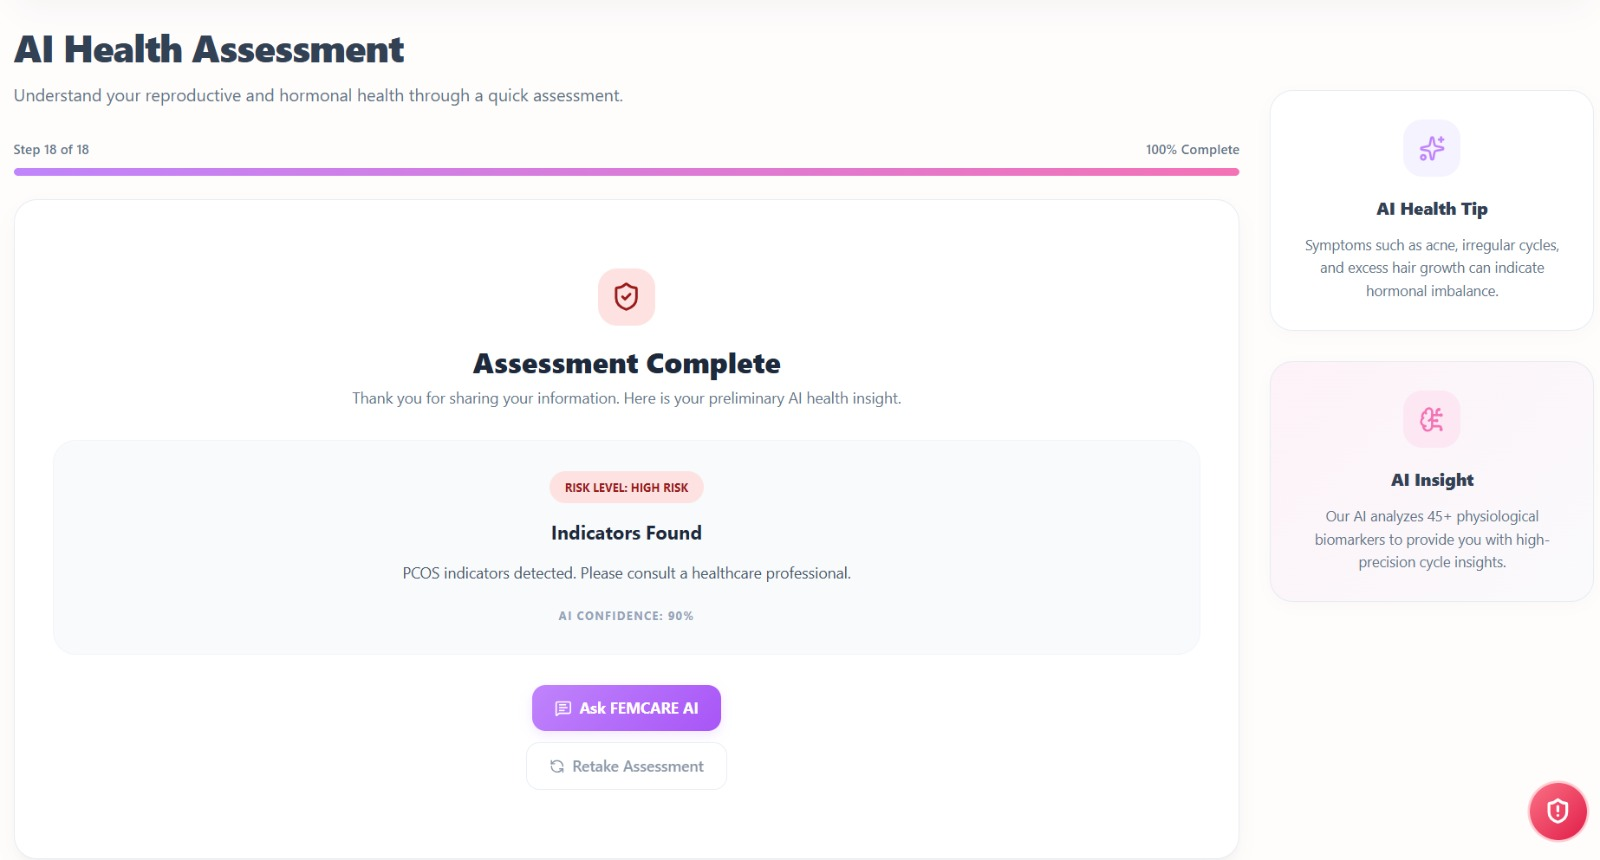
\includegraphics[width=0.8\textwidth]{assessmentphoto.jpeg}
    \caption{Caption of the figure}
    \label{fig:PCOS Assessment}
\end{figure}

\begin{table}[h!]
\centering
\caption{PCOS Assessment Test Cases}
\label{tab:tc-pcos}
\renewcommand{\arraystretch}{1.3}
\setlength{\tabcolsep}{5pt}
\begin{tabular}{|p{1cm}|p{4.5cm}|p{5cm}|p{1.5cm}|}
\hline
\rowcolor[HTML]{D9D9D9}
\textbf{ID} & \textbf{Action / Input} & \textbf{Expected Result} & \textbf{Status} \\
\hline
TC-P1 & Skip a required question and click Next & Next button remains disabled & Pass \\
\hline
TC-P2 & Leave LH, FSH, ratio fields empty and submit & Assessment submits; optional fields accepted as absent & Pass \\
\hline
TC-P3 & Enter LH = 12, FSH = 6 & Ratio auto-displays 2.00; field is read-only & Pass \\
\hline
TC-P4 & Enter LH = 10, FSH = 0 & Error message shown; no NaN or Infinity & Pass \\
\hline
TC-P5 & Enter LH = 7.5, FSH = 5 & Ratio displays 1.50 & Pass \\
\hline
TC-P6 & Submit with irregular cycles, facial hair, acne, dark patches, skipped periods & \texttt{pcos\_detected: true}; High or Moderate Risk shown & Pass \\
\hline
TC-P7 & Submit with regular cycles and no physical symptoms & \texttt{pcos\_detected: false}; Low Risk shown & Pass \\
\hline
TC-P8 & Submit while authenticated & Inputs stored in \texttt{health\_assessments}; result in \texttt{assessment\_results} & Pass \\
\hline
TC-P9 & Start backend without model file & Heuristic fallback used; same response structure returned & Pass \\
\hline
\end{tabular}
\end{table}


\begin{table}[h!]
\centering
\caption{AI Health Assistant Test Cases}
\label{tab:tc-chat}
\renewcommand{\arraystretch}{1.3}
\setlength{\tabcolsep}{5pt}
\begin{tabular}{|p{1cm}|p{4.5cm}|p{5cm}|p{1.5cm}|}
\hline
\rowcolor[HTML]{D9D9D9}
\textbf{ID} & \textbf{Action / Input} & \textbf{Expected Result} & \textbf{Status} \\
\hline
TC-CH1 & ``Why are my periods irregular?'' & Relevant health response; \texttt{scope: in\_scope} & Pass \\
\hline
TC-CH2 & ``Write Python code for sorting'' & Canned redirect message; \texttt{llm\_used: false} & Pass \\
\hline
TC-CH3 & ``I have severe sudden pain and am fainting'' & Response recommends immediate medical attention & Pass \\
\hline
TC-CH4 & Submit question from Dashboard compact chat & After reply, navigates to Community AI tab with conversation preserved & Pass \\
\hline
TC-CH5 & Click ``Ask FEMCARE AI'' from assessment result & Community AI tab opens with contextual opener referencing assessment & Pass \\
\hline
\end{tabular}
\end{table}

\subsection{Appointment Booking}
\label{subsec:tc-booking}
\begin{figure}[H]
    \centering
    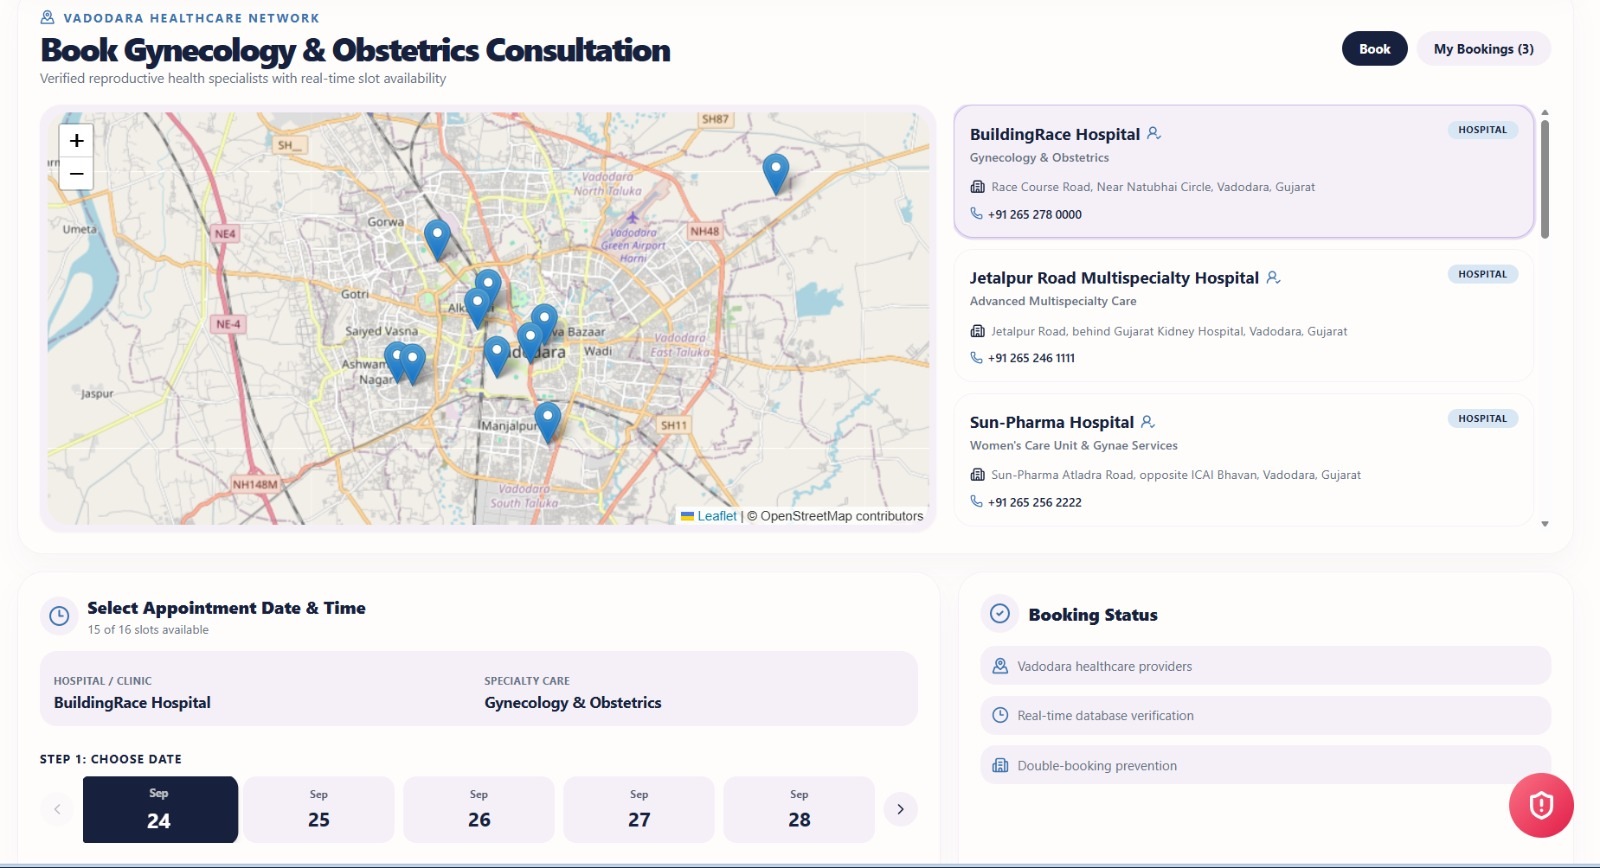
\includegraphics[width=0.8\textwidth]{slotbooking.jpeg}
    \caption{Caption of the figure}
    \label{fig:Appointment Booking}
\end{figure}

\begin{table}[h!]
\centering
\caption{Appointment Booking Test Cases}
\label{tab:tc-booking}
\renewcommand{\arraystretch}{1.3}
\setlength{\tabcolsep}{5pt}
\begin{tabular}{|p{1cm}|p{4.5cm}|p{5cm}|p{1.5cm}|}
\hline
\rowcolor[HTML]{D9D9D9}
\textbf{ID} & \textbf{Action / Input} & \textbf{Expected Result} & \textbf{Status} \\
\hline
TC-B1 & Select any provider and date & All 16 time slots rendered & Pass \\
\hline
TC-B2 & Select available slot and confirm & Booking inserted (\texttt{status = confirmed}); confirmation card with booking ID shown & Pass \\
\hline
TC-B3 & View same provider/date after TC-B2 & Booked slot disabled; 15 of 16 available & Pass \\
\hline
TC-B4 & Book same provider/date/slot as TC-B2 & HTTP 409; user informed slot is unavailable & Pass \\
\hline
TC-B5 & Cancel booking from TC-B2 & Status updated to \texttt{cancelled}; slot available again & Pass \\
\hline
TC-B6 & Book same time on a different provider & Booking accepted; constraint is per-provider & Pass \\
\hline
TC-B7 & Call \texttt{/api/book-appointment} without token & HTTP 401; no booking created & Pass \\
\hline
\end{tabular}
\end{table}

\subsection{Security and Data Isolation}
\label{subsec:tc-security}

\begin{table}[h!]
\centering
\caption{Security Test Cases}
\label{tab:tc-security}
\renewcommand{\arraystretch}{1.3}
\setlength{\tabcolsep}{5pt}
\begin{tabular}{|p{1cm}|p{4.5cm}|p{5cm}|p{1.5cm}|}
\hline
\rowcolor[HTML]{D9D9D9}
\textbf{ID} & \textbf{Action / Input} & \textbf{Expected Result} & \textbf{Status} \\
\hline
TC-S1 & Query \texttt{cycle\_logs} as User A & Only User A's rows returned & Pass \\
\hline
TC-S2 & Query \texttt{bookings} as User A & Only User A's bookings returned & Pass \\
\hline
TC-S3 & Attempt to update \texttt{assessment\_results} via client & Rejected by RLS; no update policy exists & Pass \\
\hline
TC-S4 & Simulate non-JSON backend response & \texttt{apiFetch} returns error message; no application crash & Pass \\
\hline
\end{tabular}
\end{table}

% ------------------------------------------------------------
\section{Email Notification Testing}
\label{sec:test-email}

When the Resend API key is configured, the \texttt{/health} endpoint reports \texttt{email\_enabled: true} and confirmation or cancellation emails are sent after a successful database operation. When the key is absent, \texttt{email\_enabled: false} is reported, booking operations continue to succeed, and the response includes \texttt{email\_sent: false}. The frontend displays an appropriate status message in each case without reporting a booking failure. The HTML email templates were verified by inspecting the generated output, confirming that the hospital name, formatted date, slot, status badge, and booking reference render correctly.

% ------------------------------------------------------------
\section{Observed System Results}
\label{sec:results}

The following results were observed from the running application:

\begin{itemize}
    \item All fourteen functional requirements (FR-01--FR-14 from Chapter 3) were verified as operational.
    \item The PCOS assessment returns a consistent response structure (\texttt{pcos\_detected}, \texttt{confidence}, \texttt{risk\_level}, \texttt{message}) for every valid submission, including when the heuristic fallback is active.
    \item Out-of-scope chatbot queries are rejected by the Python keyword filter without an LLM API call, verified by the \texttt{llm\_used: false} field in the response.
    \item The double-booking constraint operates at the database level and cannot be bypassed by concurrent frontend requests.
    \item Dashboard data persists correctly across browser reloads, confirming Supabase as the data source rather than transient frontend state.
  
% ------------------------------------------------------------


% ============================================================
% CHAPTER 7 -- CONCLUSION
% FEMCARE: An AI-Powered Women's Reproductive Health Platform
% ============================================================

\chapter{Conclusion}\doublespacing
\label{chap:conclusion}

This project addressed the need for an integrated digital platform that supports women in monitoring their reproductive health, understanding associated health conditions, and accessing local healthcare services. FEMCARE was designed and implemented as a full-stack web application that brings these functions together in a single authenticated system.

The platform integrates menstrual cycle tracking with real-time Dashboard visualisation, an 18-feature PCOS risk assessment using a pre-trained XGBoost classifier, and an AI health assistant that delivers topic-restricted, context-aware responses using the Groq LLM API. A Find Care module enables users to discover local women's healthcare providers, book appointments from daily time slots, and receive automated email confirmations. A Women's Health Awareness module provides searchable educational content on eight reproductive health conditions. All user data is stored in a Supabase-managed PostgreSQL database with Row Level Security enforced at the database level. Functional testing confirmed that all specified requirements operate correctly in the running application.

FEMCARE demonstrates the practical integration of machine learning, large language model assistance, cloud database management, and modern full-stack web development in a women's health application. The completed system provides a cohesive platform through which users can track their menstrual health, complete a structured PCOS assessment, obtain educational health guidance, and book consultations with local providers --- all within a single secure application. The project successfully fulfils the objectives established at the outset and delivers a functional, integrated solution to the problem it set out to address.


\chapter{Future Work}
FEMCARE is a working screening and awareness platform, but several limitations described in Chapter 3 point to clear next steps. The planned extensions are described in this chapter.

\section{Multimodal AI Health Assistant}

The current assistant accepts text input only. A planned extension is a multimodal assistant that accepts text, voice, and images, and answers within the same women's reproductive health scope.

\begin{itemize}
    \item \textbf{Voice Input and Output:} Speech-to-text would let users describe symptoms by speaking, and text-to-speech would read responses aloud. Support for Gujarati and Hindi is a priority given the intended user base in Vadodara.
    \item \textbf{Image Input:} Users could upload a photo of a skin concern such as acne or dark patches, or a photo of a lab report. Lab report images would be read using OCR to fill the LH and FSH fields automatically instead of manual entry. In the longer term, a dedicated model for ovarian ultrasound images could support the risk assessment.
    \item \textbf{Unified Pipeline:} Every input type would be converted to a common representation and passed through the existing scope check, urgency check, and user-context enrichment before the LLM is called, so the topic restriction and safety behaviour remain unchanged.
\end{itemize}

Image and voice data are more sensitive than typed answers. This extension would therefore require explicit user consent, storage protected by the same Row Level Security policies, and a clear statement that all outputs are informational and not a diagnosis.

\section{Clinical Validation and Model Improvement}

The PCOS classifier has not been independently clinically validated (Section 3.7). Future work includes testing on larger and more diverse datasets, collecting clinician-verified labels, and reporting standard metrics such as precision, recall, and AUC. Data from Indian populations would also address the generalisation concern raised in the literature survey.

\section{Explainable Predictions}

Users currently see a risk level and a confidence percentage but not the reasons behind them. Adding feature-level explanations, for example using SHAP \cite{lundberg2017}, would show which inputs contributed most to a result. This addresses the trust and explainability gap identified in Section 2.4.

\section{Privacy-Preserving Learning}

Federated learning or on-device processing could allow the model to improve over time without centralising sensitive health data. This would build on the privacy-focused approaches discussed in the literature survey.

\section{Provider and Telemedicine Features}

The Find Care module currently uses a fixed list of ten providers in Vadodara, and changing it requires a source code change. Planned improvements include:

\begin{itemize}
    \item \textbf{Admin Interface:} A dashboard for adding and editing provider details, with provider data stored in the database instead of the source code.
    \item \textbf{Provider Availability:} Working hours and days off defined by each provider, replacing the fixed sixteen daily slots.
    \item \textbf{Wider Coverage:} Providers from cities beyond Vadodara.
    \item \textbf{Video Consultation:} Online appointments through video calls, extending the platform into telemedicine, which is outside the current scope.
\end{itemize}



\chapter{Research Paper and Plagiarism Report}
\section{Paper}

\subsection*{Research Paper Introduction}

The research paper titled \textbf{``FemCare: An XGBoost-Based Platform for PCOS Risk Assessment and Menstrual Cycle Length Prediction''} presents an AI-based women's healthcare platform developed for menstrual cycle management and PCOS risk assessment. The study uses two XGBoost models: a classification model for PCOS risk assessment and a regression model for predicting menstrual cycle length. The paper also discusses menstrual tracking, mood monitoring, and gynecologist appointment support. The proposed system is designed as a decision-support tool and is not intended to replace professional medical diagnosis.

\subsection*{Research Paper Details}

\begin{itemize}
    \item \textbf{Title:} FemCare: An XGBoost-Based Platform for PCOS Risk Assessment and Menstrual Cycle Length Prediction
    
    \item \textbf{Authors:} Dhvani Milin Chokshi, Kashish Mayur Shah, Krusha Maheshbhai Paghadal, Siddhi Chiragbhai Upadhyay
    
    \item \textbf{Affiliation:} Department of Computer Science and Engineering, Parul Institute of Engineering and Technology, Parul University, Vadodara, Gujarat, India
    
    \item \textbf{Research Area:} Artificial Intelligence, Machine Learning, Women's Healthcare
    
    \item \textbf{Primary Techniques:} XGBoost Classification and XGBoost Regression
    
    \item \textbf{Paper Length:} 9 pages
    
    \item \textbf{Publication Status:} Research paper prepared for academic/research submission
\end{itemize}

\subsection*{Abstract}

FemCare is a women's healthcare platform built for menstrual cycle management and PCOS risk assessment. It uses two XGBoost models, one for PCOS risk classification and another for predicting the length of the next menstrual cycle. The study reports 99.85\% accuracy for PCOS prediction and a mean absolute error of 1.89 days for cycle-length prediction. In addition to prediction, the platform supports period and mood tracking and gynecologist appointment assistance. The system is intended as a decision-support tool rather than a diagnostic system.

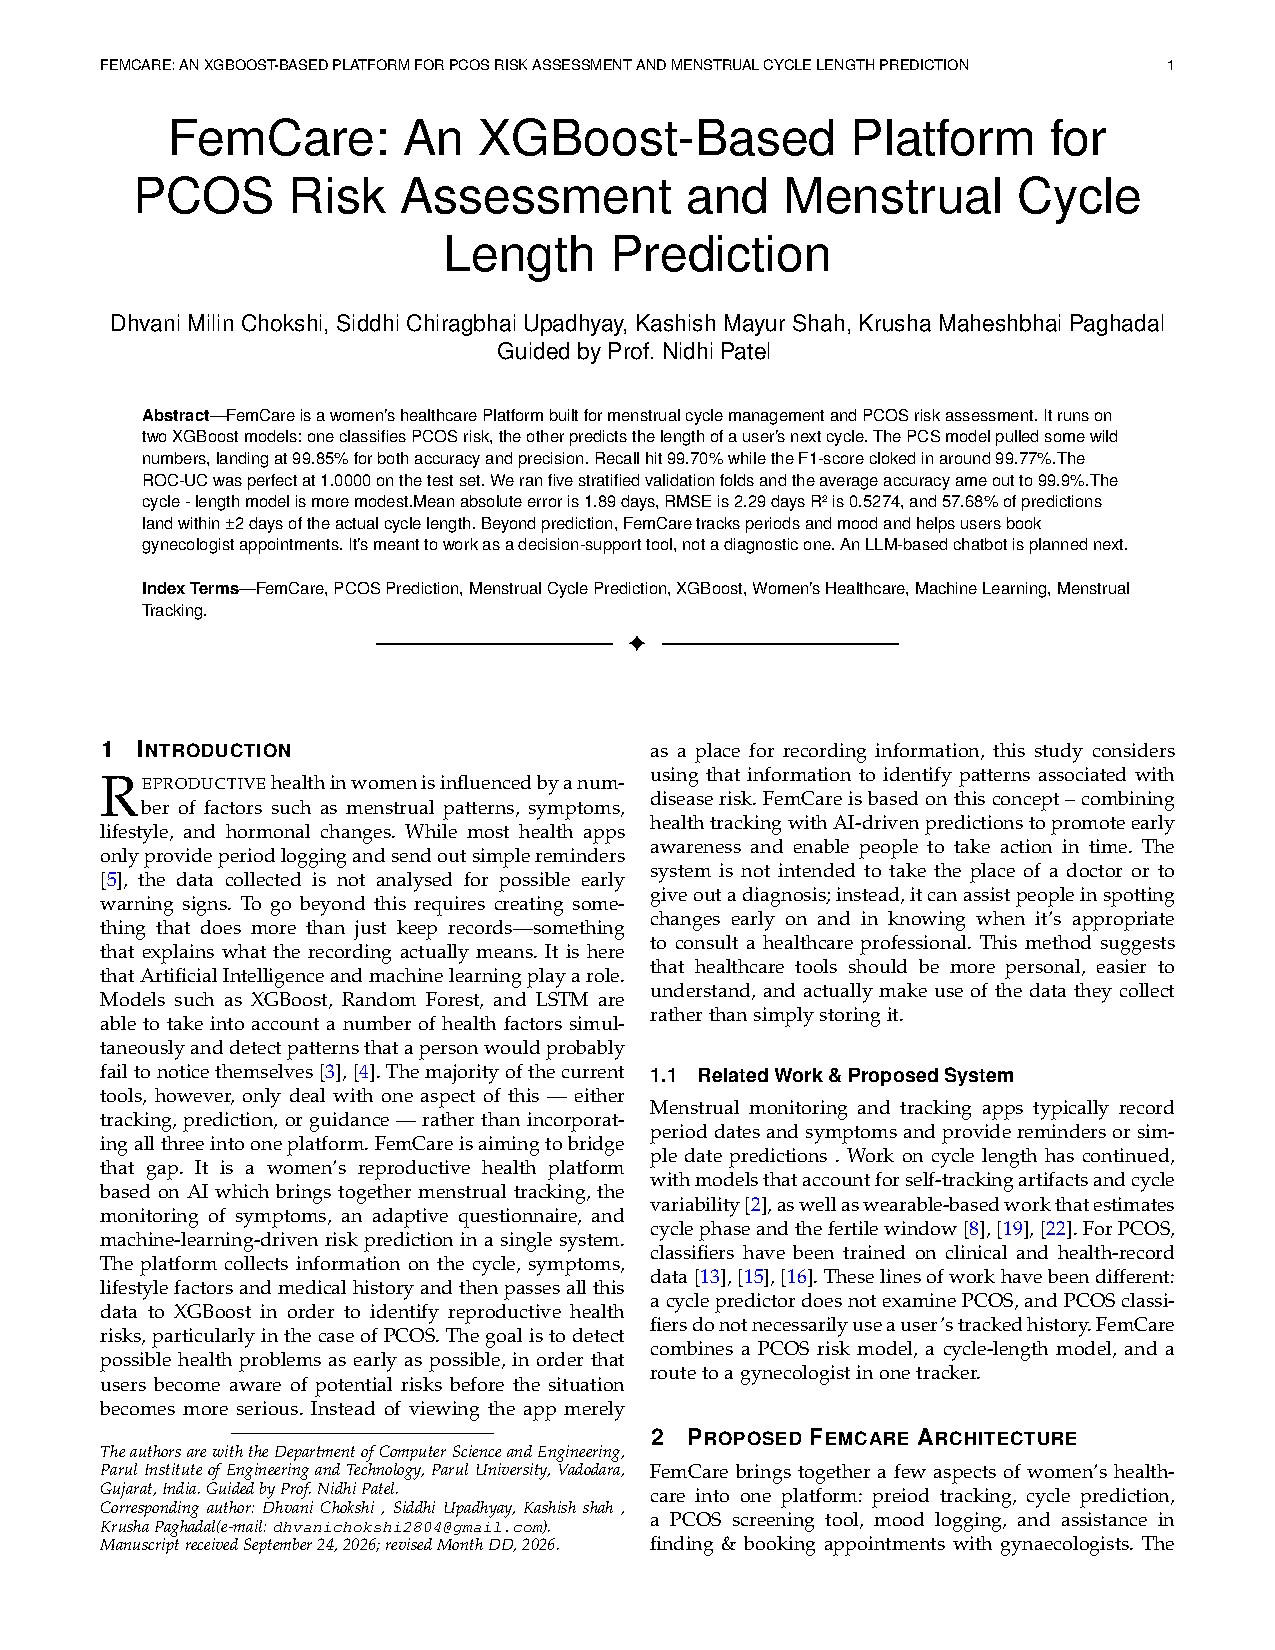
\includepdf[
    pages=-,
    fitpaper=true
]{ResearchPaper.pdf}

\section{Plagiarism and AI detection report paper}

\subsection*{Plagiarism and AI Detection Report}

The research paper was evaluated using plagiarism and AI-writing detection reports to assess the originality and writing characteristics of the submitted work. The reports were generated for the research paper titled \textbf{``FemCare: A Methodological Survey on Machine Learning Architectures for Early Detection of Polyendocrine Metabolic Outcomes''}.

\subsubsection*{Plagiarism Report}

The plagiarism assessment reported an overall similarity of \textbf{10\%}. The identified similarity consisted of matches from internet sources and published materials, while no similarity was reported from submitted student works. The report also indicates \textbf{0\% missing quotations} and \textbf{0\% missing citations}. Furthermore, the integrity overview reported \textbf{0 integrity flags}, indicating that no suspicious text manipulation was identified in the submitted document.

\subsubsection*{AI Detection Report}

The AI-writing assessment was performed on the research paper, and the report indicated \textbf{0\% AI-generated writing}. The result indicates that no AI-generated content was detected in the submitted research paper.

\subsubsection*{Report Summary}

\begin{itemize}
    \item \textbf{Overall Similarity:} 10\%
    \item \textbf{Internet Sources:} 8\%
    \item \textbf{Published Sources:} 6\%
    \item \textbf{Submitted Student Works:} 0\%
    \item \textbf{Missing Quotations:} 0\%
    \item \textbf{Missing Citations:} 0\%
    \item \textbf{Integrity Flags:} 0
    \item \textbf{AI Detection:} Below the 20\% reporting threshold; no specific percentage surfaced
\end{itemize}

The complete plagiarism report and AI detection report are attached in the following pages for reference.
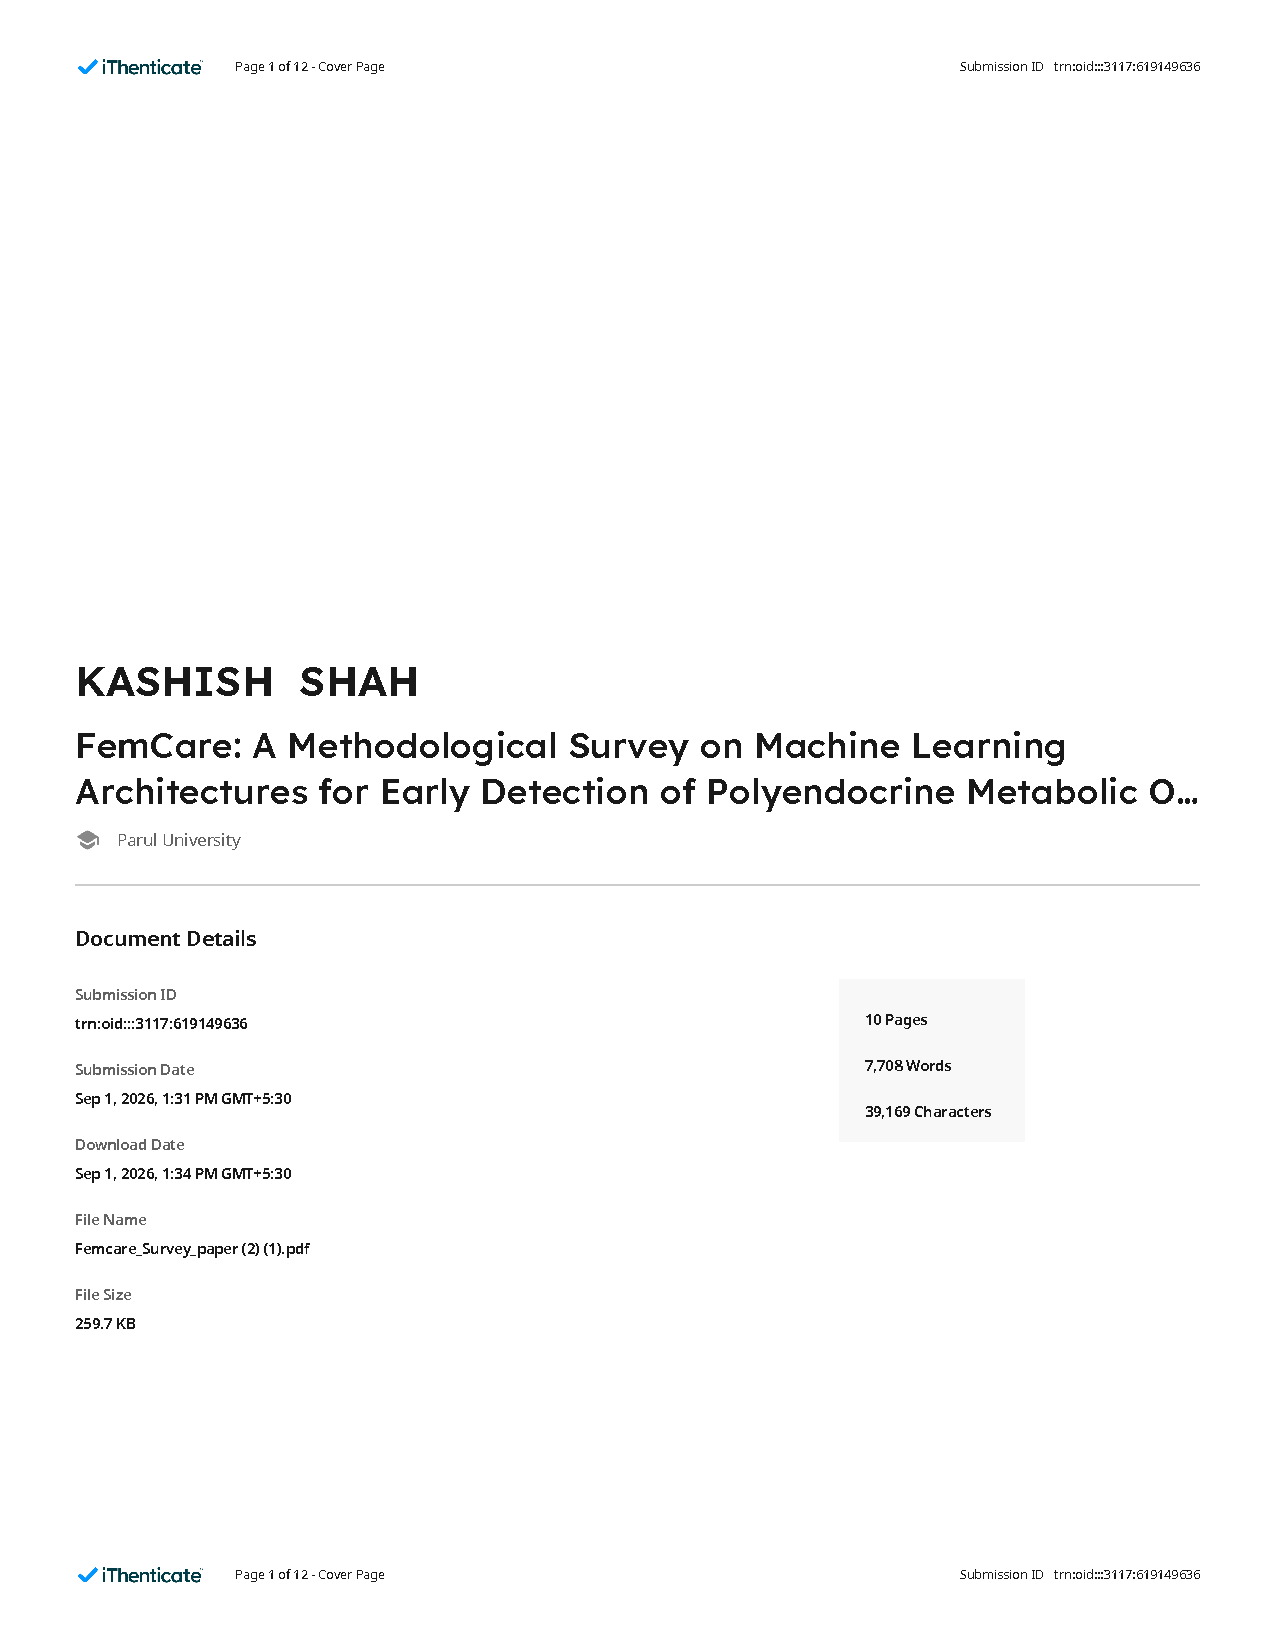
\includepdf[
    pages=-,
    fitpaper=true
]{AIdetection.pdf}

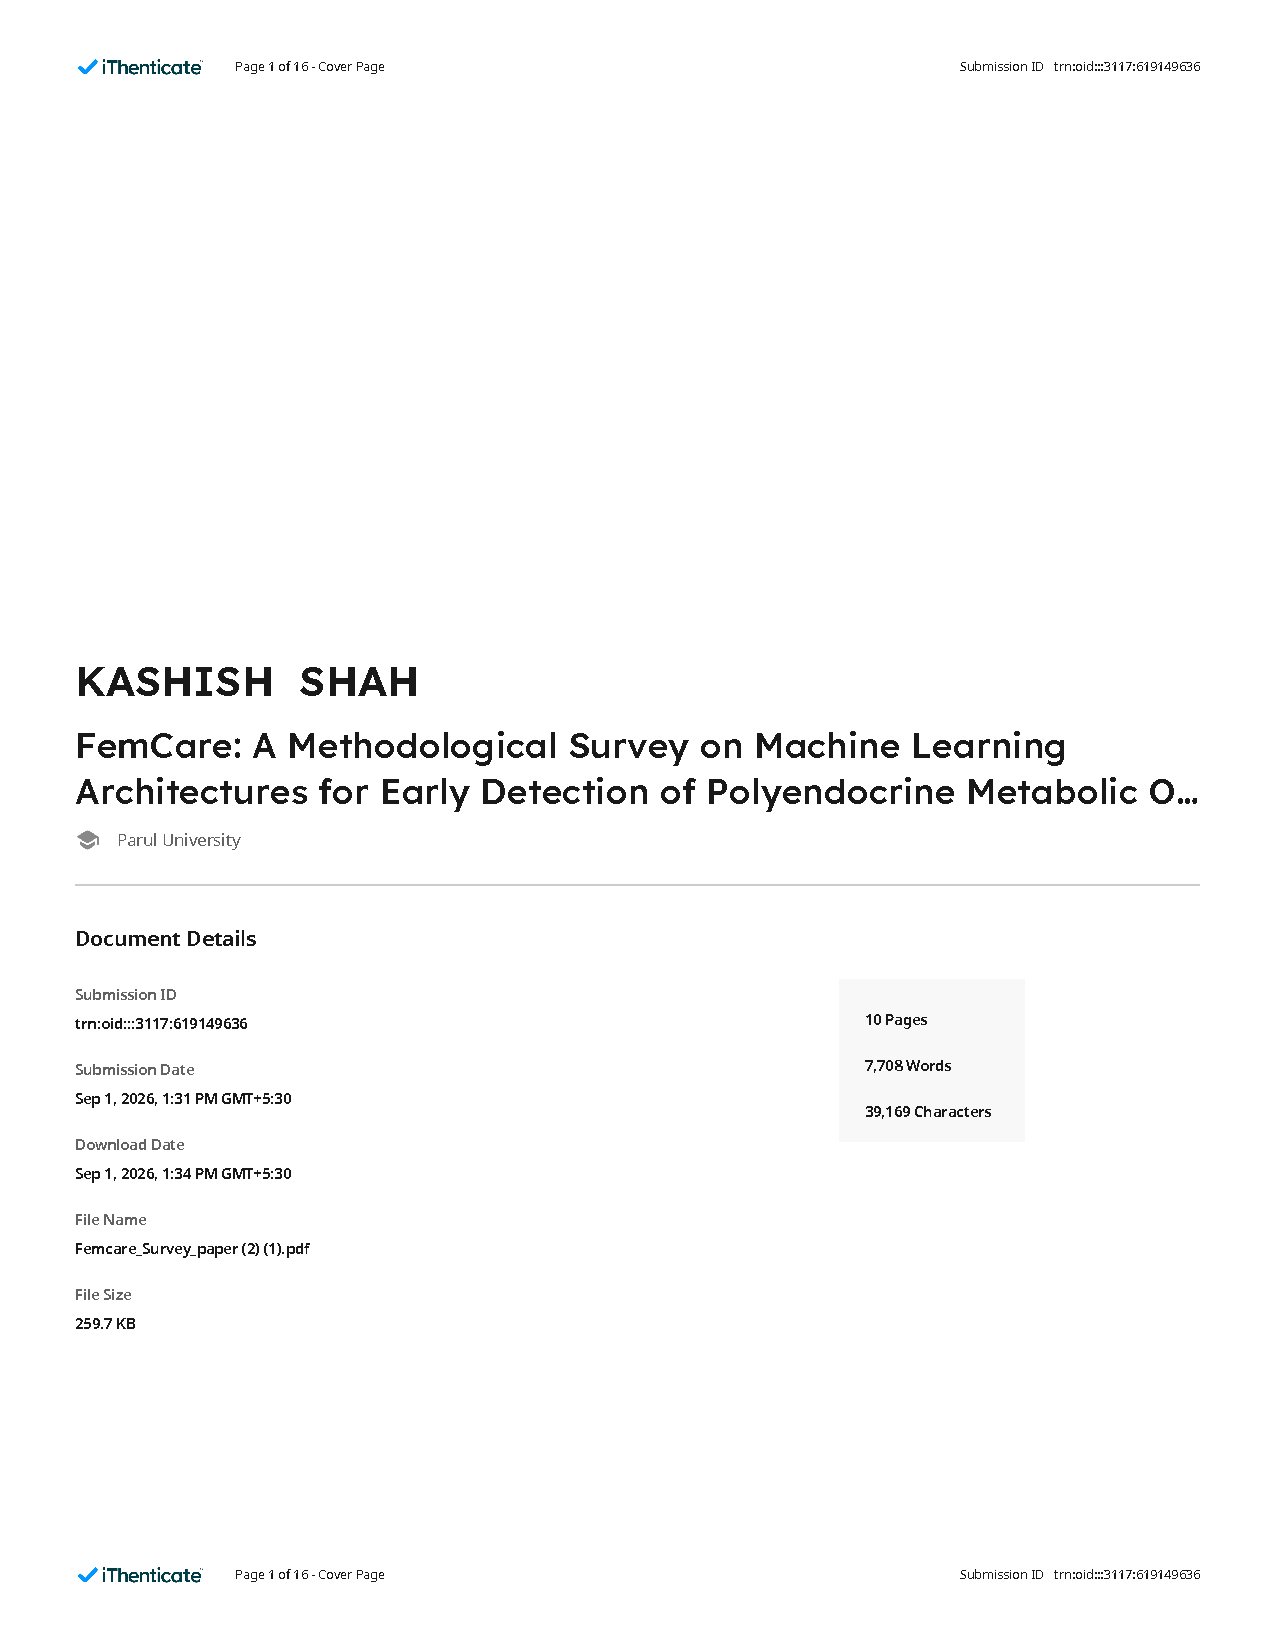
\includepdf[
    pages=-,
    fitpaper=true
]{Plagarism.pdf}




% ---------------------------------------------------------
% BIBLIOGRAPHY
% ---------------------------------------------------------

\begin{thebibliography}{00}

\bibitem{soni2025}
M. S. Soni, K. Agrawal, P. Parikh, P. Bharadva, and M. Myangar,
``Empowering college girls: From research insights to AI-based solutions
for menstrual health and academic success,''
\textit{Journal of Neonatal Surgery}, vol.~14, no.~32s,
pp.~7896--7902, 2025.

\bibitem{li2021}
K. Li, I. Urteaga, A. Shea, V. J. Vitzthum, C. H. Wiggins, and N. Elhadad,
``A generative, predictive model for menstrual cycle lengths that accounts
for potential self-tracking artifacts in mobile health data,''
arXiv preprint arXiv:2102.12439, 2021.

\bibitem{wang2024}
D. Wang and S. Zhang,
``Large language models in medical and healthcare fields: applications,
advances, and challenges,''
\textit{Artificial Intelligence Review}, vol.~57, p.~299, 2024,
doi: 10.1007/s10462-024-10921-0.

\bibitem{rossi2025}
M. Rossi and S. Rehman,
``Integrating artificial intelligence into telemedicine: Evidence, challenges,
and future directions,''
\textit{Cureus}, vol.~17, no.~8, e90829, 2025,
doi: 10.7759/cureus.90829.

\bibitem{epstein2017}
D. A. Epstein, N. B. Lee, J. H. Kang, E. Agapie, J. Schroeder,
L. R. Pina, J. Fogarty, J. A. Kientz, and S. A. Munson,
``Examining menstrual tracking to inform the design of personal informatics
tools,''
in \textit{Proceedings of the 2017 CHI Conference on Human Factors in
Computing Systems}, 2017, pp.~6876--6888,
doi: 10.1145/3025453.3025635.

\bibitem{rajesh2025}
M. Rajesh,
``Adaptive edge-federated AI framework for contactless menstrual health
prediction using multimodal physiological intelligence,''
\textit{MethodsX}, vol.~15, p.~103665, 2025,
doi: 10.1016/j.mex.2025.103665.

\bibitem{ali2023}
M. M. Ali, H. A. A. Algashamy, E. Alzidi, K. Ahmed,
F. M. Bui, S. K. Patel, S. Azam, L. F. Abdulrazak, and M. A. Moni,
``Development and performance analysis of machine learning methods for
predicting depression among menopausal women,''
\textit{Healthcare Analytics}, vol.~3, p.~100202, 2023,
doi: 10.1016/j.health.2023.100202.

\bibitem{yu2022}
J.-L. Yu, Y.-F. Su, C. Zhang, L. Jin, X.-H. Lin, L.-T. Chen,
H.-F. Huang, and Y.-T. Wu,
``Tracking of menstrual cycles and prediction of the fertile window via
measurements of basal body temperature and heart rate as well as
machine-learning algorithms,''
\textit{Reproductive Biology and Endocrinology}, vol.~20, p.~118, 2022,
doi: 10.1186/s12958-022-00993-4.

\bibitem{iturriago2025}
L. M. Iturriago-Salas, J. A. Mesa-Sarmiento, P. A. Castro-Cabrera,
A. M. \'{A}lvarez-Meza, and G. Castellanos-Dominguez,
``Artificial intelligence-driven mobile platform for thermographic imaging
to support maternal health care,''
\textit{Computers}, vol.~14, p.~466, 2025,
doi: 10.3390/computers14110466.

\bibitem{abbas2025}
Q. Abbas, W. Jeong, and S. W. Lee,
``Explainable AI in clinical decision support systems: A meta-analysis of
methods, applications, and usability challenges,''
\textit{Healthcare}, vol.~13, p.~2154, 2025,
doi: 10.3390/healthcare13172154.

\bibitem{kim2024}
H.-K. Kim,
``The effects of artificial intelligence chatbots on women's health:
A systematic review and meta-analysis,''
\textit{Healthcare}, vol.~12, p.~534, 2024,
doi: 10.3390/healthcare12050534.

\bibitem{kotz2016}
D. Kotz, C. A. Gunter, S. Kumar, and J. P. Weiner,
``Privacy and security in mobile health: A research agenda,''
\textit{Computer}, vol.~49, no.~6, pp.~22--30, 2016,
doi: 10.1109/MC.2016.185.

\bibitem{khairunisa2025}
M. Khairunisa, T. Hasanah, and R. Anwar,
``Comparison of machine learning models for menstrual cycle prediction,''
\textit{Journal of Applied Informatics and Computing}, 2025.
Available: \url{https://jurnal.polibatam.ac.id/index.php/JAIC/article/view/9076}

\bibitem{zad2024}
Z. Zad, V. S. Jiang, A. T. Wolf, T. Wang, J. J. Cheng,
I. C. Paschalidis, and S. Mahalingaiah,
``Predicting polycystic ovary syndrome with machine learning algorithms
from electronic health records,''
\textit{Frontiers in Endocrinology}, vol.~15, p.~1298628, 2024,
doi: 10.3389/fendo.2024.1298628.

\bibitem{pi2025}
X. Pi, J. Wang, L. Chu, G. Zhang, and W. Zhang,
``Prediction of high-risk pregnancy based on machine learning algorithms,''
\textit{Scientific Reports}, vol.~15, p.~15561, 2025,
doi: 10.1038/s41598-025-00450-3.

\bibitem{ahmed2023}
S. Ahmed, M. S. Rahman, I. Jahan, M. S. Kaiser,
A. S. M. S. Hosen, D. Ghimire, and S.-H. Kim,
``A review on the detection techniques of polycystic ovary syndrome
using machine learning,''
\textit{IEEE Access}, vol.~11, pp.~86522--86543, 2023,
doi: 10.1109/ACCESS.2023.3304536.

\bibitem{rahman2024}
M. M. Rahman, A. Islam, F. Islam, M. Zaman,
M. R. Islam, M. S. A. Sakib, and H. M. H. Babu,
``Empowering early detection: A web-based machine learning approach
for PCOS prediction,''
\textit{Informatics in Medicine Unlocked}, vol.~47, p.~101500, 2024,
doi: 10.1016/j.imu.2024.101500.

\bibitem{maity2025}
S. Maity and M. J. Saikia,
``Large language models in healthcare and medical applications: A review,''
\textit{Bioengineering}, vol.~12, p.~631, 2025,
doi: 10.3390/bioengineering12060631.

\bibitem{lundberg2017}
S. M. Lundberg and S.-I. Lee,
``A unified approach to interpreting model predictions,''
in \textit{Advances in Neural Information Processing Systems 30},
2017, arXiv:1705.07874.

\bibitem{goodale2019}
B. M. Goodale, M. Shilaih, L. Falco, F. Dammeier,
G. Hamvas, and B. Leeners,
``Wearable sensors reveal menses-driven changes in physiology
and enable prediction of the fertile window: Observational study,''
\textit{Journal of Medical Internet Research},
vol.~21, no.~4, p.~e13404, 2019,
doi: 10.2196/13404.

\bibitem{urteaga2017}
I. Urteaga, D. J. Albers, M. V. Wheeler, A. Druet,
H. Raffauf, and N. Elhadad,
``Towards personalized modeling of the female hormonal cycle:
Experiments with mechanistic models and Gaussian processes,''
in \textit{Advances in Neural Information Processing Systems}, 2017,
arXiv:1712.00117.

\bibitem{liu2019}
B. Liu, S. Shi, Y. Wu, D. Thomas, L. Symul,
E. Pierson, and J. Leskovec,
``Predicting pregnancy using large-scale data from a women's
health tracking mobile application,''
in \textit{Proceedings of the 2019 World Wide Web Conference
(WWW '19)}, 2019, pp.~1--7,
doi: 10.1145/3308558.3313512.

\bibitem{kilungeja2025}
G. Kilungeja, K. Graham, X. Liu, and M. Nasseri,
``Machine learning-based menstrual phase identification using
wearable device data,''
\textit{npj Women's Health}, vol.~3, p.~29, 2025,
doi: 10.1038/s44294-025-00078-8.

\bibitem{li2020}
K. Li, I. Urteaga, C. H. Wiggins, A. Druet, A. Shea,
V. J. Vitzthum, and N. Elhadad,
``Characterizing physiological and symptomatic variation in
menstrual cycles using self-tracked mobile-health data,''
\textit{Nature Digital Medicine}, vol.~3, 2020,
arXiv:1808.02932.

\bibitem{isayev2023}
A. Isayev, N. Velieva, L. Isedisha, Z. Isayeva,
K. Kamburo\u{g}lu, and F. Kuyumcu,
``Cone-beam computed tomography as a prediction tool for osteoporosis
in postmenopausal women: A systematic literature review,''
\textit{Diagnostics}, vol.~13, p.~1027, 2023,
doi: 10.3390/diagnostics13061027.

\bibitem{rego2023}
R. Rego,
``Predictive modeling of menstrual cycle length:
A time series forecasting approach,''
arXiv preprint arXiv:2308.07927, 2023.

\bibitem{dataset}
``FemCare Reproductive Health Dataset for PCOS Risk Assessment
and Menstrual Cycle Prediction,''
Published September~25, 2026.
\url{https://zenodo.org/records/22953562}.

\end{thebibliography}


% ---------------------------------------------------------
% OLD / UNUSED
% ---------------------------------------------------------

%% TITLE PAGE
\thispagestyle{empty}
%\addcontentsline{toc}{chapter}{Cover Page}\index{Cover Page}
\begin{center}
\setstretch{2}
\textcolor{purple}{{\huge \textsc{AI - driven Women’s reproductive Health & Risk Awareness
} }}\\
A Project Report \\
\vspace{0.3cm}
Submitted By\\
\vspace{0.1cm}
\textcolor{olive}{{\Large \bf Dhvani Milin Chokshi - 2303031050127}\\
{\Large \bf }}\\
\vspace{0.1cm}
\textcolor{olive}{{\Large \bf Siddhi Chiragbhai Upadhyay - 2303031050657}\\
{\Large \bf }}\\
\vspace{0.1cm}
\textcolor{olive}{{\Large \bf Kashish Mayur Shah - 2303031050547}\\
{\Large \bf }}\\
\vspace{0.1cm}
\textcolor{olive}{{\Large \bf Krusha Maheshbhai Paghadal - 2303031050320}\\
{\Large \bf }}\\
\vspace{0.1cm}
in Partial Fulfilment For the Award of\\
the Degree of\\
BACHELOR OF TECHNOLOGY\\
COMPUTER SCIENCE AND ENGINEERING\\
Under the Guidance of\\
\large{\textbf{Prof. Nidhi Mam}}\\
Your Guide Designation\\

\vspace{0.3cm}
\begin{figure}[h]
\begin{center}
     
\includegraphics[scale=0.18]{parullogo.png} \\
     \vspace{0.7cm}
     \includegraphics[scale=0.02]{Digital Use - PU NAAC Logo.jpg}
\end{center}
\end{figure}
%\textcolor{teal}{\textbf{\Huge{PARUL UNIVERSITY \\ %\textbf{NAAC A++}}}}\\
VADODARA\\
November - 2026
\end{center}

%\include{Titlepages}
%\thispagestyle{plain}
\setstretch{1.5}
%\fontfamily{qag}\selectfont
\begin{figure}
    \centering
    
\includegraphics[scale=0.15]{parullogo.png}
    \end{figure}
\vspace{1.5cm}
\begin{center}
    {\Huge \textsc{\color{violet}PARUL UNIVERSITY}}\\
   
    \vspace{1cm}
     {\Huge \bf \textsc{\color{teal}Certificate}}\\
     \vspace{0.5cm}
     \end{center}
     \large{This is to Certify that Project - II (303105423) of $7^{th}$ Semester entitled  " FemCare : AI - driven Women’s reproductive Health \& Risk Awareness ” of Group No. CSE\_35 has been successfully completed by}
     \begin{center}
\large
\begin{tabular}{l@{\hspace{6cm}}r}
Dhvani Milin Chokshi & 2303031050127\\[0.05cm]
Siddhi Chiragbhai Upadhyay & 2303031050657\\[0.05cm]
Kashish Mayur Shah & 2303031050547\\[0.05cm]
Krusha Maheshbhai Paghadal & 2303031050320
\end{tabular}
\end{center}
     \noindent
    \large {under my guidance in partial fulfillment of the Bachelor of Technology (B.Tech) in Computer Science and Engineering of Parul University in Academic Year 2026- 2027.}\\ \par
   \vspace{0.5cm}
    Date of Submission :\_\_\_\_\_\_\_\_\_\_\_\_\_\_\_\_\_\_
   
 \vspace{1.0cm}

\begin{center}
\begin{tabular*}{\textwidth}{@{\extracolsep{\fill}} c c c @{}}

\color{brown}\textbf{Prof. Nidhi Patel } &
\color{brown}\textbf{Prof. Namrata Patel} &
\color{brown}\textbf{Dr. Shailendra K Mishra} \\[0.3cm]

\textbf{Project Guide} &
\textbf{Project Coordinator} &
\textbf{Head of Department} \\[0.3cm]

\textbf{CSE, PIET} &
\textbf{CSE, PIET} &
\textbf{CSE, PIET} \\

\textbf{Parul University} &
\textbf{Parul University} &
\textbf{Parul University}

\end{tabular*}
\end{center}
   
   

%\pagenumbering{arabic}

%\pagestyle{\chaptermark}{\markboth{\chaptername \\thechapter \ -\ #1}{}}

%\renewcommand{\headrulewidth}{2pt}
%\renewcommand{\footrulewidth}{1pt}

% ---------------------------------------------------------

\end{document}